%%%%%%%%%%%%%%%%%%%%%%%%%%%%%%%%%%%%%%%%%%%%%%%%%%%%%%%%%%%%%%%%%%%%%%%%%%%%%%%%%%%%%%%%%%%%%%%%%%%%%%%%%%%%%%%
%%%%%%%%%%%%%%%%%%%%%%%%%%%%%%%%%%%%%%%%%%%%%%%%%%%%%%%%%%%%%%%%%%%%%%%%%%%%%%%%%%%%%%%%%%%%%%%%%%%%%%%%%%%%%%%
% Adapted from
% Github: https://github.com/abntex/abntex2
% André Pacheco (pacheco.comp@gmail.com)
%%%%%%%%%%%%%%%%%%%%%%%%%%%%%%%%%%%%%%%%%%%%%%%%%%%%%%%%%%%%%%%%%%%%%%%%%%%%%%%%%%%%%%%%%%%%%%%%%%%%%%%%%%%%%%%
%%%%%%%%%%%%%%%%%%%%%%%%%%%%%%%%%%%%%%%%%%%%%%%%%%%%%%%%%%%%%%%%%%%%%%%%%%%%%%%%%%%%%%%%%%%%%%%%%%%%%%%%%%%%%%%

\documentclass[12pt, openright, oneside, a4paper, english]{abntex2}

% ---
% Pacotes básicos 
% ---
\usepackage{lmodern}			% Usa a fonte Latin Modern			
\usepackage[T1]{fontenc}		% Selecao de codigos de fonte.
\usepackage[utf8]{inputenc}		% Codificacao do documento (conversão automática dos acentos)
\usepackage{lastpage}			% Usado pela Ficha catalográfica
\usepackage{indentfirst}		% Indenta o primeiro parágrafo de cada seção.
\usepackage{color}				% Controle das cores
\usepackage{graphicx}			% Inclusão de gráficos
\usepackage{microtype} 			% para melhorias de justificação
\usepackage{amsthm}
\usepackage{amsmath}
\usepackage{mathtools}
\usepackage{amsfonts}
\usepackage{amssymb}
%\usepackage{mathtools}
\usepackage{caption}
\usepackage{subcaption}
\usepackage{tabularx}
\usepackage{csquotes}
\usepackage{makecell}

% \usepackage{subfigure}

%\usepackage{kbordermatrix}
\usepackage{amsmath}

% \usepackage[portuguese,ruled,lined,linesnumbered]{algorithm2e}
\usepackage[ruled,lined,linesnumbered]{algorithm2e}
% \renewcommand{\algorithmcfname}{Algorithm}

\usepackage{multirow}

\usepackage[brazil]{babel}
\addto\captionsbrazil{%
\def\bibname{References}%
\renewcommand{\figurename}{Figure}
\renewcommand{\tablename}{Table}
\renewcommand{\listfigurename}{List of Figures}
\renewcommand{\listtablename}{List of Tables}
\renewcommand{\contentsname}{Contents}
\renewcommand\chaptername{Chapter}
}

\selectlanguage{english}


% ---
		
% ---
% Pacotes adicionais, usados apenas no âmbito do Modelo Canônico do abnteX2
% ---
\usepackage{lipsum}				% para geração de dummy text
% ---

% ---
% Pacotes de citações
% ---
%\usepackage{backref}	 % Paginas com as citações na bibl
%\usepackage[alf,abnt-and-type=&]{abntex2cite}	% Citações padrão ABNT
\usepackage[alf]{abntex2cite}	% Citações padrão ABNT
% \usepackage[style=abnt,ittitles]{biblatex}


%\newtheorem{mydef}{Definição}[chapter]

% \usepackage{natbib}

% --- 
% CONFIGURAÇÕES DE PACOTES
% --- 

% ---
% Configurações do pacote backref
% Usado sem a opção hyperpageref de backref
%\renewcommand{\backrefpagesname}{Citado na(s) página(s):~}
% Texto padrão antes do número das páginas
%\renewcommand{\backref}{}
% Define os textos da citação
%\renewcommand*{\backrefalt}[4]{
%	\ifcase #1 %
%		Nenhuma citação no texto.%
%	\or
%		Citado na página #2.%
%	\else
%		Citado #1 vezes nas páginas #2.%
%	\fi}%
% ---
\newtheorem{name}{Printed output}

\selectlanguage{english}
\renewcommand{\orientadorname}{Supervisor:}







% ---
% Informações de dados para CAPA e FOLHA DE ROSTO
% ---
\titulo{Exact Computation for\\ the Normalized Power Prior}
\autor{Eduardo Adame}
\local{Rio de Janeiro}
\data{2026}
\orientador{Luiz Max Carvalho, PhD}
\coorientador{Flávio B. Gonçalves, PhD}

\instituicao{%
 School of Applied Mathematics \\
 Fundação Getulio Vargas
  \par
 Graduate Program in Applied Mathematics and Data Science}
\tipotrabalho{Master's Thesis}
% O preambulo deve conter o tipo do trabalho, o objetivo, 
% o nome da instituição e a área de concentração 
\preambulo{Master's Thesis presented to the Graduate Program in Applied Mathematics and Data Science of the School of Applied Mathematics as a requirement to obtain the degree of Master in Applied Mathematics and Data Science.}
% ---


% ---
% Configurações de aparência do PDF final

% alterando o aspecto da cor azul
\definecolor{blue}{RGB}{41,5,195}

% informações do PDF
\makeatletter
\hypersetup{
     	%pagebackref=true,
		pdftitle={\@title}, 
		pdfauthor={\@author},
    	pdfsubject={\imprimirpreambulo},
	    pdfcreator={LaTeX with abnTeX2},
		pdfkeywords={abnt}{latex}{abntex}{abntex2}{trabalho acadêmico}, 
		colorlinks=true,       		% false: boxed links; true: colored links
    	linkcolor=blue,          	% color of internal links
    	citecolor=blue,        		% color of links to bibliography
    	filecolor=magenta,      		% color of file links
		urlcolor=blue,
		bookmarksdepth=4
}
\makeatother

% O tamanho do parágrafo é dado por:
\setlength{\parindent}{1.3cm}

% Controle do espaçamento entre um parágrafo e outro:
\setlength{\parskip}{0.2cm}  % tente também \onelineskip

% ---
% compila o indice
% ---
\makeindex

%------------------------------------------------------
%----------- Personal Definitions ---------------------
%------------------------------------------------------

\addto\captionsbrazil{
	\renewcommand{\chapterautorefname}{capítulo}
	\renewcommand{\sectionautorefname}{seção}
}	

\newcommand{\R}{\mathbb{R}}
\newcommand{\x}{\boldsymbol{x}}
\newcommand{\N}{\operatorname{Normal}}
\newcommand{\betadist}{\operatorname{Beta}}
\newcommand{\bern}{\operatorname{Bernoulli}}
\newcommand{\Uni}{\operatorname{Uniform}}
\newcommand{\Poi}{\operatorname{Poisson}}
\newcommand{\tril}{\operatorname{tril}}

\newcommand{\ev}{\mathds{E}}
\newcommand{\var}{\operatorname{Var}}
\newcommand{\cor}{\operatorname{Cor}}
\newcommand{\cov}{\operatorname{Cov}}

% \newtheorem{theorem}{Teorema}[]
% \newtheorem{proposition}{Proposição}[]

% \theoremstyle{definition}
% \newtheorem{definition}{Definition}[section]

% \theoremstyle{remark}
% \newtheorem*{remark}{Observação}
% \newtheorem{assumption}{Assumption}

\newcommand{\improve}[1]{\textcolor{red}{#1}}
\usepackage{dsfont}
\usepackage{physics}
\usepackage{algpseudocode}
\usepackage{xcolor}
\usepackage{zref-clever}
% \usepackage{algorithm2e}

\newif\ifcomments
\commentstrue % comment out to hide comments

\input{other/commands}

% Norma NBR10.520/2023 - Sobrenomes em minúsculas
% \renewcommand*{\mkbibnamefamily}[1]{#1}%

% ----
\begin{document}

% Retira espaço extra obsoleto entre as frases.
\frenchspacing 

% ----------------------------------------------------------
% ELEMENTOS PRÉ-TEXTUAIS
% ----------------------------------------------------------
\pretextual

% ---
% Capa
% ---
{\LARGE \color{red} PRELIMINARY VERSION ({\selectlanguage{english}\today})}
\imprimircapa
% ---
\cleardoublepage

% ---
% Folha de rosto
% (o * indica que haverá a ficha bibliográfica)
% ---
\imprimirfolhaderosto
% ---

% ---
% Inserir a ficha bibliografica
% ---
% \begin{fichacatalografica}
% 	\begin{figure}
% 	 \includegraphics[scale=0.9]{ficha2.pdf}
% 	\end{figure}
% \end{fichacatalografica}


% \begin{folhadeaprovacao}
%     \begin{figure}
%      \includegraphics[bb=110 0 0 750]{aprov.pdf}
%     \end{figure}
% \end{folhadeaprovacao}


% ---
% Declaração de autoria
% ---
\newpage
\begin{center}
{\ABNTEXchapterfont\Large\textsc{Statement of Authorship}}
\end{center}

\vspace*{1cm}

I hereby declare that the thesis submitted is my own work. All direct or indirect
sources used are acknowledged as references. I further declare that I have not submitted
this thesis at any other institution in order to obtain a degree. \\

% ---


\newpage
% ---
% Dedicatória
% ---
% \begin{dedicatoria}
%   \vspace*{\fill}
%   \centering
%   \noindent
%   \textit{ To anyone who has ever believed in Education as the main way to overcome adversity. } \\
%   \vspace{2cm}
%   \textit{ To the memory of Marcos Vinícius Gomes, the funniest friend I could ever have had. }
%   \vspace*{\fill}
% \end{dedicatoria}
% ---



% ---
% Agradecimentos
% ---
\begin{agradecimentos}

I would like to thank [many people]

\end{agradecimentos}
% ---

\newpage
% ---
% Epígrafe
% ---
% \begin{epigrafe}
%     \vspace*{\fill}
% 	    \begin{flushright}
%             \noindent
%             \textit{``Agora eu era o herói, e o meu cavalo só falava inglês...''}\\
%             {\tiny \itshape ``Now, I was* the hero, and my horse could only speak English...''}
            
%             From \emph{João e Maria} (1977) by Chico Buarque and Sivuca.
% 		\end{flushright}
% \end{epigrafe}


% ---
\newpage

 

 

% resumo em português
\setlength{\absparsep}{18pt} % ajusta o espaçamento dos parágrafos do resumo
\begin{resumo}[Abstract]
 \begin{otherlanguage*}{english}


In statistical modelling with historical data, a central challenge is how to effectively integrate prior evidence with current observations.
This issue is particularly pressing in clinical trials and medical applications, where using historical data can improve both the efficiency and robustness of inference.
A natural Bayesian strategy for this purpose is the use of informative priors.
Among them, the normalised power prior has attracted significant interest, as it provides a principled way to control the influence of historical information.
The method introduces a power parameter, $\eta \in [0, 1]$, that governs the degree of borrowing: $\eta = 0$ discards the past data while $\eta = 1$ fully incorporates it.
This flexibility makes the framework highly appealing in practice.
Despite its advantages, the normalised power prior induces a doubly intractable posterior: the prior itself contains a normalising constant $c_0(\eta)$ that depends on the power parameter $\eta$ and is unavailable in closed form for most models of interest, rendering standard Metropolis--Hastings inapplicable.
Existing approaches therefore rely on approximate inference methods that often lack theoretical guarantees and explicit convergence properties.
To overcome these limitations, we propose exact Markov chain Monte Carlo algorithms that avoid direct evaluation of the normalising constant ratio.
The key insight is a thermodynamic identity expressing the log-ratio of normalising constants as a tractable conditional expectation under the power prior.
Exploiting this identity, we construct non-negative unbiased estimators of the normalising constant ratio via Monte Carlo integration, which we embed within an Exchange Metropolis--Hastings scheme and a pseudo-marginal framework.
We evaluate the method on Gaussian models under varying degrees of compatibility between historical and current data.
Results demonstrate that the algorithm accurately reflects data conflict by shrinking $\eta$ when the datasets are incompatible, while recovering correct posterior behaviour when they are aligned.
Comparisons with analytical baselines confirm that our method achieves reliable estimates of both model parameters and the power parameter, with efficiency suitable for practical use.
This provides a rigorous, exact alternative to approximate approaches, offering stronger guarantees for applications such as adaptive clinical trial design.

\textbf{Keywords:} Bayesian Inference; Power Prior; Doubly Intractable Distributions; Exact MCMC; Historical Data Analysis


\end{otherlanguage*}
\end{resumo}

\newpage

\begin{resumo}[Resumo]


Na modelagem estatística com dados históricos, um desafio central é integrar efetivamente evidências prévias com observações correntes.
Essa questão é especialmente relevante em ensaios clínicos e aplicações médicas, nos quais o uso de dados históricos pode aumentar tanto a eficiência quanto a robustez da inferência.
Uma estratégia bayesiana natural para esse fim é o uso de prioris informativas.
Dentre elas, a Normalised Power Prior tem atraído interesse considerável por oferecer uma forma principiada de controlar a influência das informações históricas.
O método introduz um parâmetro de potência, $\eta \in [0, 1]$, que governa o grau de incorporação: $\eta = 0$ descarta os dados passados, ao passo que $\eta = 1$ os incorpora integralmente.
Essa flexibilidade torna o arcabouço bastante atraente na prática.
Apesar de suas vantagens, a Normalised Power Prior induz uma posteriori duplamente intratável: a priori em si contém uma constante normalizadora $c_0(\eta)$ que depende do parâmetro de potência $\eta$ e não está disponível em forma fechada para a maioria dos modelos de interesse, inviabilizando a aplicação direta do algoritmo Metropolis--Hastings padrão.
As abordagens existentes dependem, portanto, de métodos de inferência aproximada que frequentemente carecem de garantias teóricas e propriedades de convergência explícitas.
Para superar essas limitações, propomos algoritmos exatos de Markov chain Monte Carlo que evitam a avaliação direta da razão de constantes de normalização.
A ideia central é uma identidade termodinâmica que expressa a log-razão das constantes de normalização como uma esperança condicional tratável sob a power prior.
Explorando essa identidade, construímos estimadores não negativos e não viesados da razão de constantes de normalização via integração de Monte Carlo, os quais são incorporados em um esquema Exchange Metropolis--Hastings e em um método pseudo-marginal.
Avaliamos o método em modelos gaussianos sob diferentes graus de compatibilidade entre dados históricos e correntes.
Os resultados demonstram que o algoritmo reflete adequadamente o conflito entre os dados ao encolher $\eta$ quando os conjuntos são incompatíveis, ao mesmo tempo que recupera o comportamento \textit{a posteriori} correto quando estão alinhados.
Comparações com referenciais analíticos confirmam que o método obtém estimativas confiáveis tanto dos parâmetros do modelo quanto do parâmetro de potência, com eficiência adequada ao uso prático.
Isso fornece uma alternativa exata e rigorosa às abordagens aproximadas, oferecendo garantias mais sólidas para aplicações como o planejamento adaptativo de ensaios clínicos.

\textbf{Palavras-chave:} Inferência Bayesiana; Power Prior; Distribuições Duplamente Intratáveis; MCMC Exato; Análise de Dados Históricos

\end{resumo}

\newpage


% ---
% inserir lista de ilustrações
% ---
\pdfbookmark[0]{\listfigurename}{lof}
\listoffigures*
\cleardoublepage
% ---

% ---
% inserir lista de tabelas
% ---
\pdfbookmark[0]{\listtablename}{lot}
\listoftables*
\cleardoublepage
% ---
%\begin{siglas}
  %\item[MSE] Erro médio quadrático
  %\item[FLR] Relacionamento Lógico Fuzzy
%\end{siglas}

% ---
% inserir o sumario
% ---
\pdfbookmark[0]{\contentsname}{toc}
\tableofcontents*
\cleardoublepage
% ---

% ----------------------------------------------------------
% ELEMENTOS TEXTUAIS
% ----------------------------------------------------------
\textual

% ----------------------------------------------------------
% Introdução (exemplo de capítulo sem numeração, mas presente no Sumário)
% ----------------------------------------------------------
\chapter{Introduction}

\label{sec:intro}

\comLM{Second-to-last thing to be written. Don't sweat it. Leave it to \textit{Papa}
\begin{itemize}
    \item Describe NPP and notation; motivation with historical data (MANY CITATIONS).
    \item The NPP as a doubly-intractable problem (the prior is intractable)
    \item Mention that we start with approximate methods and then move on to exact stuff
\end{itemize}
}

% Here we talk about informative priors
In statistical modelling with historical data, a central challenge is effectively integrating information from past studies with current data.
This is particularly relevant in clinical trials and medical research, where leveraging historical data can improve the efficiency and robustness of statistical inferences.
A natural approach in this setting is the use of \textit{informative priors}, which incorporate prior knowledge into the analysis, thereby enhancing parameter estimation and decision-making \cite{spiegelhalter2004, gelman2013, ibrahim2015}.

% Here we talk about power priors
Among the various methods for constructing informative priors, \textit{power priors} \cite{ibrahim2000, ibrahim2015} have gained significant attention.
They allow for controlled borrowing of information from historical data by adjusting a power parameter, $\eta$, which typically ranges between 0 and 1.
When $\eta = 0$, no historical information is incorporated, whereas $\eta = 1$ fully integrates the historical data into the current analysis.
This flexibility makes power priors particularly appealing in adaptive clinical trial design and other settings where historical evidence is available, but its relevance is uncertain.

However, when $\eta$ is itself treated as unknown and assigned a prior distribution, the resulting posterior is \textit{doubly intractable}: the normalised power prior contains a normalising constant $c_0(\eta)$ that depends on $\eta$ and cannot be evaluated in closed form for general likelihoods, preventing direct use of Metropolis--Hastings.
Current approaches rely on \textit{approximate methods} \cite{carvalho2021} that lack theoretical guarantees and explicit convergence bounds.
This work addresses this gap by developing exact Markov chain Monte Carlo algorithms \cite{murray2012, goncalves2017, vats2021} that avoid evaluating the intractable normalising constant ratio altogether, providing a rigorous computational baseline for inference under the normalised power prior.



\chapter{Background}

\section{Bayesian Inference}

\subsection{Principles}

Bayesian inference provides a probabilistic framework for updating uncertainty about unknown quantities after observing data.

Let $D$ denote the observed data, and let $\theta \in \Theta$ denote an unknown parameter defined on a measurable parameter space $(\Theta,\mathcal{F})$.
The Bayesian model is specified by a likelihood function $L(D\mid\theta)$ and a prior distribution $\pi_0(\theta)$.

The likelihood describes the information about $\theta$ contained in the data, while the prior represents information available before observing $D$.
Bayes' theorem combines these two sources of information through the posterior distribution

\begin{equation}
    \pi(\theta\mid D)
    =
    \frac{L(D\mid\theta)\pi_0(\theta)}
    {\int_{\Theta} L(D\mid t)\pi_0(t)\,\dd t}.
    \label{eq:bayes-theorem-background}
\end{equation}

The denominator in \eqref{eq:bayes-theorem-background} is the marginal likelihood, or evidence, and is given by

\begin{equation}
    m(D)
    =
    \int_{\Theta} L(D\mid t)\pi_0(t)\,\dd t.
    \label{eq:marginal-likelihood-background}
\end{equation}

When $m(D)<\infty$, the posterior distribution is well-defined and integrates to one.
In this sense, Bayesian inference can be understood as a normalization procedure that transforms the unnormalized density $L(D\mid\theta)\pi_0(\theta)$ into a probability distribution over $\Theta$.

For any posterior-integrable function $h:\Theta\to\bR$, posterior summaries are often expressed through expectations of the form

\begin{equation}
    \bE_{\pi(\theta\mid D)}\qty[h(\theta)]
    =
    \int_{\Theta} h(\theta)\pi(\theta\mid D)\,\dd\theta.
    \label{eq:posterior-expectation-background}
\end{equation}

Examples include posterior means, posterior variances, marginal probabilities, credible intervals, and posterior predictive quantities.
The main computational challenge is that the posterior distribution is usually available only up to a normalizing constant.

Indeed, many Bayesian algorithms only require the unnormalized posterior density

\begin{equation}
    \gamma(\theta)
    =
    L(D\mid\theta)\pi_0(\theta),
    \label{eq:unnormalized-posterior-background}
\end{equation}

because the marginal likelihood $m(D)$ does not depend on $\theta$.

However, the marginal likelihood is still important for model comparison, empirical Bayes procedures, and doubly intractable models.
In low-dimensional conjugate models, the integral in \eqref{eq:marginal-likelihood-background} may be available analytically.

In modern Bayesian models, this integral is often unavailable, and posterior expectations such as \eqref{eq:posterior-expectation-background} must be approximated numerically. This motivates the use of simulation-based methods.

\subsection{Monte Carlo Methods}

Monte Carlo methods approximate integrals by random sampling.

Let $\pi$ be a probability distribution on $(\Theta,\mathcal{F})$, and suppose that the quantity of interest is

\begin{equation}
    \mu
    =
    \bE_{\pi}\qty[h(\theta)]
    =
    \int_{\Theta} h(\theta)\pi(\theta)\,\dd\theta.
    \label{eq:mc-target-background}
\end{equation}

If $\theta_1,\dots,\theta_N$ are independent samples from $\pi$, then the Monte Carlo estimator of $\mu$ is

\begin{equation}
    \widehat{\mu}_N
    =
    \frac{1}{N}\sum_{i=1}^{N} h(\theta_i).
    \label{eq:mc-estimator-background}
\end{equation}

Under standard integrability conditions, the law of large numbers gives

\begin{equation}
    \widehat{\mu}_N
    \xrightarrow[N\to\infty]{a.s.}
    \mu.
    \label{eq:mc-lln-background}
\end{equation}

If $h(\theta)$ has finite variance under $\pi$, the central limit theorem gives

\begin{equation}
    \sqrt{N}\qty(\widehat{\mu}_N-\mu)
    \xrightarrow[N\to\infty]{d}
    \mathcal{N}\qty(0,\sigma_h^2),
    \label{eq:mc-clt-background}
\end{equation}

where

\begin{equation}
    \sigma_h^2
    =
    \operatorname{Var}_{\pi}\qty[h(\theta)].
    \label{eq:mc-variance-background}
\end{equation}

The important feature of the Monte Carlo approximation is that its convergence rate is typically $N^{-1/2}$ and does not directly depend on the dimension of $\Theta$.
This makes Monte Carlo methods attractive for Bayesian inference, where posterior distributions are often high-dimensional.

The difficulty is that independent sampling from $\pi(\theta\mid D)$ is rarely possible.
Markov chain Monte Carlo methods address this difficulty by constructing a Markov chain whose invariant distribution is the desired posterior distribution.

The samples are then dependent, but posterior expectations can still be estimated using ergodic averages.
If $(\theta_n)_{n\geq 0}$ is a Markov chain with invariant distribution $\pi$, then the MCMC estimator is

\begin{equation}
    \widehat{\mu}_N^{\operatorname{MCMC}}
    =
    \frac{1}{N}\sum_{n=1}^{N} h(\theta_n).
    \label{eq:mcmc-estimator-background}
\end{equation}

Under suitable irreducibility, recurrence, and integrability conditions, the ergodic theorem gives

\begin{equation}
    \widehat{\mu}_N^{\operatorname{MCMC}}
    \xrightarrow[N\to\infty]{a.s.}
    \bE_{\pi}\qty[h(\theta)].
    \label{eq:mcmc-ergodic-theorem-background}
\end{equation}

The price paid for replacing independent samples with a Markov chain is autocorrelation.

When samples are correlated, the effective amount of information in $N$ iterations may be much smaller than $N$ independent draws.
This motivates the use of diagnostics such as effective sample size, Monte Carlo standard errors, trace plots, and comparisons across independent chains.
Another important practical issue is initialization.

A Markov chain usually starts from a distribution different from $\pi$, and therefore the early iterations may not be representative of the target distribution.
The usual practical response is to discard an initial portion of the chain, known as burn-in.

However, burn-in is an asymptotic correction rather than an exact one.
This distinction is central to the later discussion of exact and unbiased MCMC methods.

\section{Standard MCMC Methods}
\comEA{Since I know you will ask me what do I mean by standard: we can surely think of a better name}

\subsection{Gibbs Sampling}

\subsection{Metropolis-Hastings}

\section{Doubly Intractable Distributions}
\label{sec:dbl-int}

\section{The Normalized Power Prior}

\subsection{Formulation}

Consider the following Bayesian schema:

\begin{equation}
    p(\theta \mid D) = \dfrac{L(D \mid \theta) \pi_{0}(\theta)}{\int_{\Theta} L(D \mid t) \pi(t) \, \dd t} = \dfrac{L(D \mid \theta) \overbrace{\pi_{0}(\theta)}^{\text{Initial prior}}}{m(D)}.
\end{equation}


\begin{defi}[Power prior]
    Let $D_0 = \{d_{01}, d_{02}, \dots, d_{0N_0}\}$, $d_{0i} \subseteq \cX^{p}$ be the historical data and let $L_0(D_0 \mid \theta)$ be a likelihood function assumed to be finite for all $\theta \in \Theta \subseteq \bR^p$. Then, the power prior is defined as

    \begin{equation}
        \label{eq:power-prior}
        \pi_\eta(\theta \mid D_0) \propto L_0(D_0 \mid \theta)^{\eta} \pi_0(\theta),
    \end{equation}

    where $\pi_0(\theta)$ is the initial prior distribution of $\theta$ and $\eta$ is the (fixed) power parameter.
\end{defi}

Then, when we want to accomodate the uncertainty in the choice of $\eta$, we treat it as a random variable and assign a prior distribution to it, indexed by $\phi$. In this case, we find the \textit{unnormalized} power prior as

\begin{equation}
    \pi^\star(\theta, \eta \mid D_0, \phi) = \pi_\eta(\theta \mid D_0) \pi_A(\eta \mid \phi) \propto L_0(D_0 \mid \theta)^{\eta} \pi_0(\theta) \pi_A(\eta \mid \phi).
\end{equation}

In order to compute the posterior distribution of $\theta$ and $\eta$, we need to find the normalizing constant (from \eqref{eq:power-prior}) $c_0(\eta)$, which is given by

\begin{equation}
    \label{eq:normalizing-constant}
    c_0(\eta) = \int_{\Theta} L_0(D_0 \mid t)^{\eta}\,  \dd P_0(t)
\end{equation}

and the marginal posterior distribution of $\eta$ as, for a new dataset $D$,

\begin{equation}
    p(\eta \mid D, D_0, \phi) \propto \dfrac{\pi_A(\eta \mid \phi)}{c_0(\eta)} \int_{\Theta} L(D \mid t) L_0(D_0 \mid t)^{\eta} \, \dd P_0(t).
\end{equation}


Notice that, since both \( c_0(\eta) \) and \( \int_{\Theta} L(D \mid t) L_0(D_0 \mid t)^{\eta} \, \dd P_0(t) \) are intractable, we call this a doubly-intractable posterior. Previous work \cite{adame2025, carvalho2021} have focused on emulating \( \log c_0(\eta) \) and \( \log c'(\eta) = \bE_{\pi_\eta}\qty[\log L_0(D_0\mid \theta)] \) \eqref{eq:normalizing-constant-log} through non-parametric models, which has proven to be more effective than common interpolation methods—particularly when incorporating shape constraints.

Sampling from these posteriors is challenging due to the intractability of standard M-H acceptance probabilities, making approximate methods like auxiliary variable techniques computationally expensive and lacking convergence guarantees; an alternative is unbiased event constructions, which enable exact sampling without evaluating normalizing constants.

For instance, applying Barker's algorithm for MCMC~\cite{vats2021} to sample from a target distribution \( \pi(x) \propto \pi'(x) \) with proposal density \( q(x\mid y) \) has become feasible through Bernoulli factory methods. These methods enable the construction of events with probability \( \alpha_B(x, y) \) when
\begin{equation}
\alpha_B(x, y) = \dfrac{\pi(y)q(y\mid x)}{\pi(x)q(x\mid y) + \pi(y)q(y\mid x)} = \dfrac{\pi'(y)q(y\mid x)}{\pi'(x)q(x\mid y) + \pi'(y)q(y\mid x)}
\end{equation}
cannot be directly evaluated~\cite{goncalves2017}.

\subsection{Properties}

\subsubsection{Derivative of the normalizing constant}

Considering $c_0(\eta)$ as in \eqref{eq:normalizing-constant}, we can find the derivative of $c_0(\eta)$ with respect to $\eta$ as

\begin{align*}
    \dfrac{\dd c_0(\eta)}{\dd \eta} &= \dfrac{\dd}{\dd \eta} \int_{\Theta} L(D_0 \mid t)^{\eta}\,  \dd P_0(t), \\
    &= \int_{\Theta} \dfrac{\dd}{\dd \eta} L(D_0 \mid t)^{\eta}\,  \dd P_0(t), \\
    &= \int_{\Theta} \log(L(D_0 \mid t)) L(D_0 \mid t)^{\eta}\,  \dd P_0(t), \\
    &= \int_{\Theta} \log(L(D_0 \mid t)) \pi_\eta(t \mid D_0)\,  \dd P_0(t), \\
    &= c_0(\eta)\bE_{\pi_\eta}[\log(L(D_0 \mid \theta))],
\end{align*}

where $\bE_{\pi_\eta}[\cdot]$ denotes the expectation with respect to the power prior distribution $\pi_\eta(\theta \mid D_0)$.

When we're interested on the derivative of the logarithm of the normalizing constant, we can use the following expression:

\begin{align}
    \label{eq:normalizing-constant-log}
    \dfrac{\dd \log c_0(\eta)}{\dd \eta} &= \dfrac{1}{c_0(\eta)}\dfrac{\dd c_0(\eta)}{\dd \eta} = \bE_{\pi_\eta}[\log(L(D_0 \mid \theta))].
\end{align}


\subsection{Other Historical Data Modelling Approaches}


\section{Unbiased MCMC Methods}

\subsection{Barker's Algorithm for Exact Inference}

Barker's algorithm \cite{barker1965} provides an alternative to Metropolis-Hastings that is amenable to Bernoulli factory methods.
For a target distribution $\pi(\theta)$ and proposal $q(\theta'|\theta)$, Barker's acceptance probability is:
\begin{equation}
\alpha_B(\theta, \theta') = \frac{\pi(\theta') q(\theta|\theta')}{\pi(\theta) q(\theta'|\theta) + \pi(\theta') q(\theta|\theta')}
\end{equation}

While Barker's algorithm has lower efficiency than Metropolis-Hastings in the Peskun ordering, its acceptance probability has a crucial property: it can be expressed as a ratio of products.
This enables the use of \textit{Bernoulli factory} methods to implement the acceptance decision without explicitly computing $\alpha_B$.

\subsubsection{The Two-Coin Algorithm}

The fundamental building block is the two-coin algorithm \cite{goncalves2017}.
Suppose we can factorize the acceptance odds as:
\begin{equation}
\frac{\pi(\theta') q(\theta|\theta')}{\pi(\theta) q(\theta'|\theta)} = \frac{c(\theta', \theta) p(\theta', \theta)}{c(\theta, \theta') p(\theta, \theta')}
\end{equation}
where $c(\cdot, \cdot)$ is tractable and $p(\cdot, \cdot) \in [0,1]$ is a probability we can simulate.

Then, Barker's acceptance probability becomes:
\begin{equation}
\alpha_B(\theta, \theta') = \frac{c(\theta', \theta) p(\theta', \theta)}{c(\theta', \theta) p(\theta', \theta) + c(\theta, \theta') p(\theta, \theta')}
\end{equation}

The two-coin algorithm generates this probability without computing it explicitly:

\begin{algorithm}[H]
    % \label{alg:twocoin}
        Flip coins with probabilities $p(\theta', \theta)$ and $p(\theta, \theta')$\;
        \uIf{both heads or both tails}{
        return to step 1\;
        }
        \uElseIf{first heads and second tails}{
        accept (return 1)\;
        }
        \uElseIf{first tails and second heads}{
        reject (return 0)\;
        }
    \caption{Two-coin algorithm \froyo{Just the idea}}
\end{algorithm}

This procedure produces an acceptance event with exactly probability $\alpha_B(\theta, \theta')$.

\subsection{Divide-and-Conquer Bernoulli Factory (DCBF)}

For models with $n$ observations, the likelihood factorizes as $\pi(\theta|D) \propto \prod_{i=1}^n f_i(\theta)$.
The vanilla two-coin algorithm requires flipping a coin with probability $p(\theta) = \prod_{i=1}^n p_i(\theta)$.
As $n$ grows, $p(\theta)$ shrinks exponentially, causing the expected number of loops (ENL) to grow as $O(e^{cn})$ for some constant $c > 0$.
This exponential cost is prohibitive even for moderate $n$

\subsubsection{The Coin Merge Procedure}

The DCBF addresses this by hierarchically merging factor coins.
For two factors with odds $h_1, h_2$ and corresponding probabilities $r_j = h_j/(h_j + g_j)$, we can merge them into a single coin with probability $r_0 = h_0/(h_0 + g_0)$ where $h_0 = h_1 h_2$.


\begin{algorithm}[H]
    Flip coins with probabilities $r_1$ and $r_2$\;
    \eIf{both return the same value (both 0 or both 1)} 
    {return that value\;}
    {return to step 1\;}
\caption{Coin merge algorithm \froyo{Just the idea (again)}}
\label{alg:coinmerge}
\end{algorithm}

\subsubsection{Hierarchical Factorization}

Given $n$ factors, we organize them in a balanced binary tree of depth $\ell = \lceil \log_2 n \rceil$.

At the leaves, we place individual factors (or small batches).
At each internal node, we merge the coins from its two children.

\begin{algorithm}[H]
    \SetKwProg{Fn}{function}{}{end}
    \Fn{FlipDCBF($\{f_1, \ldots, f_n\}$, level $k$)}
    {
        \If{$n = 1$}{\KwRet Flip2Coin($f_1$)\;}
        Split factors into $\{f_1, \ldots, f_{n/2}\}$ and $\{f_{n/2+1}, \ldots, f_n\}$\;
        $c_1 \gets$ FlipDCBF(left half, $k+1$)\;
        $c_2 \gets$ FlipDCBF(right half, $k+1$)\;
        \KwRet MergeCoins($c_1$, $c_2$)\;
        }
\caption{Divide-and-Conquer Bernoulli Factory}
\end{algorithm}

\subsubsection{Computational Complexity}

\cite{stumpf2025} prove that under regularity conditions, the expected cost of the DCBF scales as:
\begin{equation}
\bE[\text{Cost}] = O(4^\ell \cdot \rho(n, \ell))
\end{equation}
where $\rho(n, \ell)$ is the cost of the two-coin algorithm at the leaves with batch size $n/2^\ell$.

For posterior concentration at rate $n^{-1/2}$ with optimal proposal scaling:
\begin{itemize}
\item If using likelihood ratio estimators: $\rho(n, \ell) = O(\sqrt{n/2^\ell})$
\item Setting $4^\ell \propto n$ gives overall cost $O(n^{3/2})$
\end{itemize}

This is polynomial, compared to the exponential $O(e^{cn})$ cost of vanilla two-coin.

Moreover, this matches or improves upon pseudo-marginal algorithms, which typically require $O(n^2)$ cost.

\subsection{Pseudo-marginal Metropolis-Hastings}

\section{Function Emulation Methods}

\subsection{Gaussian Processes}


\subsection{Generalized Additive Models}

\subsection{Shape-constrained Variants}

\chapter{Approximate inference with noisy-MCMC}
\label{chap:approximate}


Current approaches:
\begin{itemize}
    \item Function emulation: \cite{adame2025, carvalho2021}
\end{itemize}

\comLM{\cite{han2023} \cite{carvalho2021} and references therein }

\comLM{Need to carefully read, cite and discuss \cite{park2020}. Do their results hold for SCAM, for instance?}


Our contributions in this area:
\begin{itemize}
    \item Do MaL estimation and talk about GP and SCAM;
    \item Importance sampling to simplify and improve estimation of the NPP normalising constant (including control variates);
    \item Showcase on moderate size examples (including NIG linear regression as a baseline). Show that it works and then show how to break it    
\end{itemize}


\section{Emulating the normalizing constant}

In many applications involving normalized power priors, the normalizing constant

\begin{equation}
    c_0(\eta)
    =
    \int_{\Theta}
    L(D_0 \mid \theta)^\eta
    \pi_0(\theta)
    \dd \theta
\end{equation}

cannot be evaluated analytically.
As a consequence, direct evaluation of the posterior density becomes infeasible.
A common strategy is therefore to replace $c_0(\eta)$ by a surrogate approximation constructed from evaluations at a finite collection of design points.

More precisely, suppose we evaluate the log-normalizing constant

\begin{equation}
    g(\eta)
    =
    \log c_0(\eta)
\end{equation}

at points $\eta_1, \ldots, \eta_m \in [0,1]$.
The evaluations may be obtained analytically, via Monte Carlo estimators, thermodynamic integration, or path sampling methods.
We then construct an emulator

\begin{equation}
    \widehat g(\eta)
\end{equation}

intended to approximate $g(\eta)$ over the entire interval.
This yields the approximation

\begin{equation}
    c_0(\eta)
    \approx
    \exp\{\widehat g(\eta)\}.
\end{equation}

The resulting approximation can then be plugged into the posterior density, producing an approximate MCMC scheme whose computational cost is substantially reduced after the emulator is trained.

From a statistical perspective, this transforms the problem of evaluating an intractable normalizing constant into a nonparametric regression problem.
The quality of inference then depends on the approximation properties of the emulator and on how uncertainty propagates through the posterior distribution.

\subsection{Consequences}

Although emulation methods can dramatically reduce computational cost, replacing the true normalizing constant by a deterministic approximation may substantially alter the resulting posterior distribution.

Suppose the true posterior density is

\begin{equation}
    \pi(\theta, \eta \mid D, D_0)
    \propto
    \frac{
        L(D \mid \theta)
        L(D_0 \mid \theta)^\eta
        \pi_0(\theta)
        \pi_0(\eta)
    }{
        c_0(\eta)
    }.
\end{equation}

If $c_0(\eta)$ is replaced by an approximation $\widehat c_0(\eta)$, the resulting Markov chain targets instead

\begin{equation}
    \widetilde \pi(\theta, \eta \mid D, D_0)
    \propto
    \frac{
        L(D \mid \theta)
        L(D_0 \mid \theta)^\eta
        \pi_0(\theta)
        \pi_0(\eta)
    }{
        \widehat c_0(\eta)
    }.
\end{equation}

Consequently, approximation errors directly perturb the invariant distribution of the Markov chain.
Even small systematic biases in $\widehat c_0(\eta)$ may produce substantial distortions in posterior summaries, credible intervals, and Bayes factors.

An important practical issue is that many emulation approaches treat $\widehat c_0(\eta)$ as deterministic after fitting.
In this case, uncertainty associated with the emulator is ignored during posterior inference.
This may lead to overconfident posterior distributions and unreliable uncertainty quantification.

The problem becomes particularly severe when the approximation error varies non-uniformly across the parameter space.
For instance, local interpolation errors near regions of high posterior mass may induce systematic bias in the marginal posterior distribution of $\eta$.

Moreover, unconstrained emulators may violate structural properties known to hold for the true function.
For normalized power priors, the map

\begin{equation}
    g(\eta)
    =
    \log c_0(\eta)
\end{equation}

typically satisfies smoothness and monotonicity properties inherited from the likelihood.
Approximations that ignore such information may generate unrealistic artifacts, including oscillations and locally inconsistent curvature.

These issues motivate the incorporation of structural constraints into the emulation procedure.

\subsection{Introducing shape-constraints}

One strategy for improving the stability of the emulator is to incorporate qualitative information about the target function directly into the model.

Suppose

\begin{equation}
    g(\eta)
    =
    \log c_0(\eta).
\end{equation}

Under regularity conditions, derivatives of $g$ can be expressed in terms of moments under the power posterior distribution.
For instance,

\begin{equation}
    \dv{}{\,\eta}
    \log c_0(\eta)
    =
    \bE_{\pi_\eta}
    \qty[
        \log L(D_0 \mid \theta)
    ].
\end{equation}

Therefore, information about monotonicity and curvature may be available analytically or estimated from Monte Carlo samples.

A flexible approach consists of modelling $g$ as a Gaussian process.
If

\begin{equation}
    g
    \sim
    \mathcal{GP}(m, k),
\end{equation}

then derivatives of $g$ are also Gaussian processes because differentiation is a linear operator.
In particular,

\begin{equation}
    g'
    \sim
    \mathcal{GP}
    \qty(
        \dv{}{\,\eta} m(\eta),
        \dv{}{\,\eta}\dv{}{\,\eta'} k(\eta, \eta')
    ).
\end{equation}

This allows derivative information and shape restrictions to be incorporated directly into the posterior distribution of the Gaussian process.
Conditioning on derivative observations or derivative sign constraints can substantially reduce unrealistic oscillatory behaviour.
We refer to \citeonline{adame2025} for recent developments in shape-constrained emulation through Gaussian processes.
\comEA{Insert more references}

An alternative strategy is based on shape-constrained additive models (SCAMs).
These models extend generalized additive models (GAMs) by imposing constraints directly on the spline basis coefficients.

Suppose

\begin{equation}
    g(\eta)
    =
    \beta_0
    +
    \sum_{j=1}^p
    f_j(\eta),
\end{equation}

where the functions $f_j$ are represented through spline expansions.
Shape constraints such as monotonicity or convexity can then be enforced by restricting the spline coefficients during estimation.

In practice, SCAMs are fitted using penalized likelihood methods analogous to standard GAM estimation procedures.
The main difference is that the optimization is performed under linear inequality constraints on the spline coefficients.

Compared with unconstrained smoothers, shape-constrained models may provide more stable extrapolation behaviour and improved uncertainty quantification in regions with sparse design points.
These properties are particularly appealing when approximating normalizing constants, since small local errors may propagate nonlinearly into the posterior distribution.

\section{Current approaches for the NPP}
\comEA{Discuss \cite{han2023} and \cite{carvalho2021} - and any other state-of-art}

\section{Doubly Intractable Settings}

\comEA{Discuss \cite{park2020}}

Doubly intractable distributions arise in Bayesian inference when the likelihood takes the form
\begin{equation}
\pi(\theta \mid x) \propto p(\theta)\frac{h(x \mid \theta)}{Z(\theta)},
\end{equation}
where the normalizing constant $Z(\theta)$ depends on the parameter $\theta$ and cannot be evaluated pointwise, as discussed in detail on seciton \ref{sec:dbl-int}.
This setting is common in models such as exponential random graph models, Markov point processes, and, more generally, in likelihoods derived from Gibbs measures.
In the context of Normalized Power Priors (NPP), this issue naturally appears due to the presence of parameter-dependent normalizing constants, making standard Bayesian computation challenging.

A number of Markov chain Monte Carlo (MCMC) methods have been proposed to address this problem, including auxiliary variable approaches such as the exchange algorithm and the double Metropolis--Hastings (DMH) algorithm. While these methods can target the exact posterior distribution, they typically require simulating auxiliary variables at each iteration, which becomes computationally prohibitive in high-dimensional or complex models.

An alternative strategy is proposed by \citeonline{park2020}, who introduce a function emulation approach to approximate the intractable normalizing constant. Their method replaces repeated Monte Carlo estimation of $Z(\theta)$ with a two-stage surrogate model.
First, importance sampling is used to obtain noisy estimates of $Z(\theta)$ at a finite set of parameter values.
Then, a Gaussian process (GP) is fitted to the log-normalizing function, providing a fast interpolator that can be evaluated within an MCMC algorithm.
This leads to two variants: one that emulates only the normalizing function (NormEm), and another that emulates the entire likelihood (LikEm).

The main advantage of this approach is computational efficiency.
By shifting the costly Monte Carlo approximations to a precomputation stage, the resulting MCMC algorithm avoids repeated simulation of auxiliary variables, yielding substantial speed-ups compared to exact or pseudo-marginal methods.
Moreover, the approach is naturally parallelizable and extends beyond doubly intractable settings to more general problems involving expensive likelihood evaluations.

However, this efficiency comes at the cost of asymptotic exactness.
The resulting Markov chain targets an approximate posterior distribution, with an error that depends on both the number of importance samples and the number of design points used to train the Gaussian process.
While theoretical bounds on the total variation distance are provided, they do not yield explicit rates, making it difficult to calibrate the approximation in practice.

Several additional limitations remain. First, the method relies on importance sampling estimates, which can exhibit high variance in moderate to high-dimensional settings, potentially degrading the quality of the surrogate.
Second, the Gaussian process approximation assumes a smooth structure for the log-normalizing function and typically ignores heteroskedasticity induced by Monte Carlo noise.
Third, the selection of design points (particles) is critical but performed using heuristic procedures such as short runs of DMH or approximate Bayesian computation, without a principled adaptive strategy.
Finally, the approach does not scale well with the dimension of the parameter space due to the cubic complexity of Gaussian process regression and the increasing difficulty of covering the parameter space.

These limitations suggest several directions for future research.
In particular, combining surrogate-based approximations with exact correction mechanisms, such as pseudo-marginal or delayed-acceptance schemes, could potentially recover asymptotic exactness while retaining computational gains.
Additionally, replacing importance sampling with more robust estimators, and incorporating adaptive or local surrogate models, may improve both stability and scalability.
Such developments are particularly relevant in the context of NPP models, where efficient and reliable inference remains an open challenge.

\chapter{Exact inference for the Normalised Power Prior}
\label{sec:exact}

In this chapter, we develop exact Markov chain Monte Carlo methods for inference under the normalised power prior.

The full joint posterior of interest is
\begin{equation}
    \pi(\theta, \eta \mid D, D_0)
    \propto
    L(D \mid \theta)\,
    \frac{L_0(D_0 \mid \theta)^{\eta}\, \pi_0(\theta)}{c_0(\eta)}\,
    \pi_A(\eta),
    \label{eq:full-posterior-exact}
\end{equation}
and the central challenge is the intractable ratio $c_0(\eta)/c_0(\eta')$ that appears in any Metropolis--Hastings update of $\eta$.

We address this challenge through three complementary constructions: the exchange algorithm (Section~\ref{sec:exact-exchange}), the Poisson estimator (Section~\ref{subsec:poisson-estimator}), and a pseudo-marginal approach based on importance sampling (Section~\ref{sec:pseudo-marginal-is}).

Updating $\theta$ given $(\eta, D, D_0)$ is straightforward: the full conditional
\begin{equation}
    \pi(\theta \mid \eta, D, D_0) \propto L(D \mid \theta)\, L_0(D_0 \mid \theta)^{\eta}\, \pi_0(\theta)
    \label{eq:theta-full-conditional}
\end{equation}
does not involve $c_0(\eta)$, so standard Metropolis--Hastings (Section~\ref{subsec:metropolis}) applies directly.

For a symmetric proposal $q(\theta' \mid \theta) = q(\theta \mid \theta')$, the acceptance ratio reduces to
\begin{equation}
    \alpha(\theta, \theta' \mid \eta)
    =
    \min\!\left\{1,\,
    \frac{L(D \mid \theta')\,\pi_0(\theta')}{L(D \mid \theta)\,\pi_0(\theta)}
    \left(\frac{L_0(D_0 \mid \theta')}{L_0(D_0 \mid \theta)}\right)^{\!\eta}
    \right\}.
\end{equation}

The remainder of this chapter focuses on the harder problem of updating $\eta$.

\section{Exchange Metropolis--Hastings}
\label{sec:exact-exchange}

Applying the exchange algorithm of Section~\ref{subsec:exchange-algorithm} to the NPP, the intractable quantity is $c_0(\eta)$ as defined in \eqref{eq:normalising-constant}.
\begin{equation}
c_0(\eta)
=
\int_\Theta L_0(D_0 \mid \theta)^\eta \pi_0(\theta) \dd \theta.
\end{equation}

If the current value of $\theta$ is fixed and a proposal $\eta'$ is generated from $q(\eta' \mid \eta)$, the exchange update draws
\begin{equation}
\theta^\star
\sim
\pi_{\eta'}(\theta \mid D_0)
=
\frac{L_0(D_0 \mid \theta)^{\eta'}\pi_0(\theta)}
{c_0(\eta')}.
\end{equation}
The exchange ratio for the $\eta$ update is then
\begin{align}
R_{\mathrm{ex}}(\eta,\eta';\theta,\theta^\star)
&=
\frac{\pi_A(\eta')}{\pi_A(\eta)}
\frac{q(\eta \mid \eta')}{q(\eta' \mid \eta)}
\frac{L_0(D_0 \mid \theta)^{\eta'-\eta}}
{L_0(D_0 \mid \theta^\star)^{\eta'-\eta}}.
\end{align}
The ratio $c_0(\eta)/c_0(\eta')$ has disappeared.
This cancellation is the main reason why the exchange algorithm is attractive for the normalised power prior.

According to the exchange algorithm framework of \citeonline{murray2012}, the auxiliary draw from $\pi_{\eta'}(\theta \mid D_0)$ introduces a factor $1/c_0(\eta')$ into the augmented target that exactly cancels the intractable ratio (see Appendix~\ref{proof:exchange-correctness} for a self-contained argument).

The exactness of the exchange algorithm depends on the ability to sample $\theta^\star$ exactly from $\pi_{\eta'}(\theta \mid D_0)$.
This assumption is strong.
It is satisfied in conjugate Gaussian models and in some conditionally conjugate models.
It is not automatically satisfied in general regression models or in non-conjugate likelihoods.
If $\theta^\star$ is generated by an inner MCMC chain that is not run to stationarity, the resulting algorithm is no longer exactly the exchange algorithm.
In that case, the method becomes an approximate exchange or double Metropolis--Hastings algorithm.

\section{Barker's method via Poisson estimator}

Updating $\eta$ is more delicate because the full conditional
\begin{equation}
    \pi(\eta \mid \theta, D, D_0) \propto \frac{\pi_A(\eta)}{c_0(\eta)}\, L_0(D_0 \mid \theta)^{\eta}
    \label{eq:eta-full-conditional}
\end{equation}
involves $c_0(\eta)$ explicitly.

The Metropolis--Hastings ratio for a proposal $\eta \to \eta'$ is
\begin{equation}
    \frac{\pi(\eta' \mid \theta)}{\pi(\eta \mid \theta)}
    =
    \frac{\pi_A(\eta')}{\pi_A(\eta)}
    \cdot
    \frac{c_0(\eta)}{c_0(\eta')}
    \cdot
    L_0(D_0 \mid \theta)^{\eta' - \eta},
\end{equation}
and the intractable ratio $c_0(\eta)/c_0(\eta')$ prevents direct evaluation.

Recalling the thermodynamic identity established in \eqref{eq:normalising-constant-log}, integrating from $\eta$ to $\eta'$ gives
\begin{equation}
    \label{eq:log-ratio-integral}
    \Delta(\eta, \eta')
    \coloneqq
    \log\frac{c_0(\eta')}{c_0(\eta)}
    =
    \int_{\eta}^{\eta'}
    \bE_{\pi_\tau}\bigl[\log L_0(D_0 \mid \theta)\bigr]
    \,\dd\tau,
\end{equation}
where $\pi_\tau(\theta) \propto L_0(D_0 \mid \theta)^\tau \pi_0(\theta)$ is the power prior at temperature $\tau$.

The goal of the following sections is to construct a non-negative unbiased estimator of $\exp\{-\Delta(\eta,\eta')\} = c_0(\eta)/c_0(\eta')$.


\subsection{Producing an unbiased estimator via a Poisson estimator}
\label{subsec:poisson-estimator}

Let $\pi_\tau$ denote the power posterior associated with the historical data.
For $\tau\in[0,1]$, define
\begin{equation}
    \pi_\tau(\theta)
    =
    \frac{L_0(D_0\mid \theta)^\tau \pi_0(\theta)}
    {c_0(\tau)},
    \qquad
    c_0(\tau)
    =
    \int_\Theta L_0(D_0\mid t)^\tau \,\dd P_0(t).
\end{equation}
For two values $\eta,\eta'\in[0,1]$, define
\begin{equation}
    \Delta(\eta,\eta')
    =
    \log\frac{c_0(\eta')}{c_0(\eta)}.
\end{equation}
Under the usual regularity conditions allowing differentiation under the integral sign, the thermodynamic identity gives
% Identity is proved in Appendix~\ref{proof:deriv-normalising-constant}.
\begin{equation}
    \Delta(\eta,\eta')
    =
    \int_{\eta}^{\eta'}
    \bE_{\theta\sim \pi_\tau}
    \left[
        \log L_0(D_0\mid \theta)
    \right]
    \,\dd \tau.
\end{equation}
Equivalently, if $U\sim\mathrm{Unif}(0,1)$ and $\tau_{\eta,\eta'}(U)=\eta+U(\eta'-\eta)$, then
\begin{equation}
    \Delta(\eta,\eta')
    =
    \bE_{U}
    \left[
        (\eta'-\eta)
        \bE_{\theta\sim \pi_{\tau_{\eta,\eta'}(U)}}
        \{\log L_0(D_0\mid \theta)\}
    \right].
\end{equation}

This representation suggests a proposal-specific random variable.
Let $\mathsf P_{\eta,\eta'}$ be the probability measure on $[0,1]\times\Theta$ obtained by first drawing $U\sim\mathrm{Unif}(0,1)$ and then drawing $\theta\sim\pi_{\tau_{\eta,\eta'}(U)}$.
Equivalently,
\begin{equation}
    \mathsf P_{\eta,\eta'}(\dd u,\dd\theta)
    =
    \dd u\,
    \pi_{\tau_{\eta,\eta'}(u)}(\dd\theta).
\end{equation}
Define
\begin{equation}
    Z_{\eta,\eta'}(U,\theta)
    =
    (\eta'-\eta)\log L_0(D_0\mid \theta).
\end{equation}
Then
\begin{equation}
    \bE_{\mathsf P_{\eta,\eta'}}[Z_{\eta,\eta'}]
    =
    \Delta(\eta,\eta').
\end{equation}

The objective is to construct an unbiased estimator of the ratio $c_0(\eta)/c_0(\eta')$.
This ratio can be written as
\begin{equation}
    \exp\{-\Delta(\eta,\eta')\}
    =
    \frac{c_0(\eta)}{c_0(\eta')}.
\end{equation}
Assume that there exist deterministic constants $a_{\eta,\eta'}$ and $b_{\eta,\eta'}$ such that
\begin{equation}
    a_{\eta,\eta'}
    \le
    Z_{\eta,\eta'}(U,\theta)
    \le
    b_{\eta,\eta'}
    \qquad
    \mathsf P_{\eta,\eta'}\text{-almost surely}.
\end{equation}
Set
\begin{equation}
    c_{\eta,\eta'}
    =
    b_{\eta,\eta'},
    \qquad
    \lambda_{\eta,\eta'}
    =
    b_{\eta,\eta'}-a_{\eta,\eta'}.
\end{equation}
Draw $K\sim\mathrm{Poisson}(\lambda_{\eta,\eta'})$.
Conditionally on $K$, draw
\begin{equation}
    (U_j,\theta_j)_{j=1}^K
    \overset{\mathrm{iid}}{\sim}
    \mathsf P_{\eta,\eta'}.
\end{equation}
The Poisson estimator is
\begin{equation}
    \widehat I(\eta,\eta')
    =
    \exp\{\lambda_{\eta,\eta'}-c_{\eta,\eta'}\}
    \prod_{j=1}^{K}
    \frac{
        c_{\eta,\eta'} -
        Z_{\eta,\eta'}(U_j,\theta_j)
    }{
        \lambda_{\eta,\eta'}
    }.
    \label{eq:poisson-estimator}
\end{equation}
By construction, each factor satisfies
\begin{equation}
    0
    \le
    \frac{
        c_{\eta,\eta'} -
        Z_{\eta,\eta'}(U_j,\theta_j)
    }{
        \lambda_{\eta,\eta'}
    }
    \le
    1.
\end{equation}
Therefore $\widehat I(\eta,\eta')$ is non-negative.
\begin{proof}
    
Using the exponential formula for a Poisson random variable, we obtain
\begin{align}
    \bE[\widehat I(\eta,\eta')]
    &=
    \exp\{\lambda_{\eta,\eta'}-c_{\eta,\eta'}\}
    \bE\left[
        \left\{
        \bE_{\mathsf P_{\eta,\eta'}}
        \left[
        \frac{c_{\eta,\eta'}-Z_{\eta,\eta'}}{\lambda_{\eta,\eta'}}
        \right]
        \right\}^K
    \right] \\
    &=
    \exp\{\lambda_{\eta,\eta'}-c_{\eta,\eta'}\}
    \exp\left\{
        \lambda_{\eta,\eta'}
        \left(
        \frac{c_{\eta,\eta'}-\Delta(\eta,\eta')}
             {\lambda_{\eta,\eta'}}
        -1
        \right)
    \right\} \\
    &=
    \exp\{-\Delta(\eta,\eta')\}.
\end{align}
Thus, $\widehat I(\eta,\eta')$ is an unbiased estimator of the normalising-constant ratio $c_0(\eta)/c_0(\eta')$.
\end{proof}

The efficiency of the estimator depends strongly on the envelope width $\lambda_{\eta,\eta'}=b_{\eta,\eta'}-a_{\eta,\eta'}$.
Large envelopes lead to large Poisson counts and high estimator variability.
Therefore, the practical usefulness of the construction depends on obtaining deterministic but sufficiently tight proposal-specific bounds for $Z_{\eta,\eta'}$.

It is important to distinguish this unbiased estimator from an exact Barker accept--reject mechanism.
Although $\widehat I(\eta,\eta')$ is unbiased for $c_0(\eta)/c_0(\eta')$, substituting a noisy estimate of the likelihood ratio directly into the Barker probability does not generally produce an exact Barker transition.
Exact Barker implementations require simulating the accept--reject event itself with the correct marginal probability, typically through a Bernoulli-factory or two-coin construction.

\subsubsection{Practical implementation}

The integral $\Delta(\eta,\eta')$ in \eqref{eq:log-ratio-integral} is estimated by Monte Carlo.

Drawing $\tau_k \overset{\mathrm{iid}}{\sim} \mathrm{Unif}(\eta,\eta')$ and, conditionally, $\widetilde{\theta}_{m,k} \sim \pi_{\tau_k}$ for $m = 1,\ldots,M$ and $k = 1,\ldots,K$, gives the double Monte Carlo estimator
\begin{equation}
    \widehat{\Delta}(\eta, \eta')
    =
    \frac{(\eta' - \eta)}{MK}
    \sum_{k=1}^{K} \sum_{m=1}^{M}
    \log L_0\bigl(D_0 \mid \widetilde{\theta}_{m,k}\bigr).
\end{equation}
This is an unbiased estimator of $\Delta(\eta,\eta')$ by the law of total expectation.

In the single-draw case ($K = M = 1$), this reduces to
\begin{equation}
    \label{eq:single-draw-delta}
    \widehat{\Delta}(\eta, \eta') = (\eta' - \eta)\,\log L_0(D_0 \mid \widetilde{\theta}_\star),
    \qquad
    \tau_\star \sim \mathrm{Unif}(\eta,\eta'),
    \quad
    \widetilde{\theta}_\star \sim \pi_{\tau_\star},
\end{equation}
which can be used in the Poisson estimator construction of Section~\ref{subsec:poisson-estimator}.

Note that only the mean of $Z_{\eta,\eta'}$, not its variance, enters the unbiasedness argument; the variance governs the efficiency of the estimator through the expected Poisson count $\lambda_{\eta,\eta'}$.

\subsection{Local envelopes for the Poisson estimator}
\label{subsec:local-envelopes}

The preceding construction does not require a single global envelope that is valid uniformly over all possible proposals.
Instead, for each proposed move $\eta\to\eta'$, it is enough to obtain deterministic bounds for the proposal-specific random variable
\begin{equation}
    Z_{\eta,\eta'}(U,\theta)
    =
    (\eta'-\eta)\log L_0(D_0\mid \theta),
    \qquad
    (U,\theta)\sim\mathsf P_{\eta,\eta'}.
\end{equation}
Suppose that the historical log-likelihood satisfies
\begin{equation}
    \ell_{\min}
    \le
    \log L_0(D_0\mid\theta)
    \le
    \ell_{\max}
    \qquad
    \text{for all }\theta\in\Theta.
\end{equation}
Then, for a fixed proposal $\eta\to\eta'$, define
\begin{equation}
    a_{\eta,\eta'}
    =
    \min\{(\eta'-\eta)\ell_{\min},
          (\eta'-\eta)\ell_{\max}\}.
\end{equation}
Similarly, define
\begin{equation}
    b_{\eta,\eta'}
    =
    \max\{(\eta'-\eta)\ell_{\min},
          (\eta'-\eta)\ell_{\max}\}.
\end{equation}
The resulting envelope width is
\begin{equation}
    b_{\eta,\eta'}-a_{\eta,\eta'}
    =
    |\eta'-\eta|(\ell_{\max}-\ell_{\min}).
\end{equation}
Hence a natural local choice is
\begin{equation}
    c_{\eta,\eta'}
    =
    b_{\eta,\eta'},
    \qquad
    \lambda_{\eta,\eta'}
    =
    |\eta'-\eta|(\ell_{\max}-\ell_{\min}).
\end{equation}
This choice makes the expected number of Poisson factors proportional to the proposal distance $|\eta'-\eta|$.
Consequently, local random-walk proposals in $\eta$ lead to smaller expected computational cost than large independent proposals.

For unbounded parameter spaces, such as Gaussian models with $\Theta=\mathds{R}^d$, the lower bound $\ell_{\min}$ is typically $-\infty$.
In that case, the above exact Poisson construction is not directly applicable without additional structure.
One possible solution is to work with a compactly supported prior.
For example, define
\begin{equation}
    \pi_{0,B}(\theta)
    \propto
    \pi_0(\theta)\mathbf 1_{\Theta_B}(\theta),
\end{equation}
where $\Theta_B\subset\Theta$ is compact.
Then deterministic bounds for $\log L_0(D_0\mid\theta)$ can be derived on $\Theta_B$.
In the Gaussian historical likelihood with known covariance, the log-likelihood is a concave quadratic function of $\theta$.
Its maximum is attained at the historical maximum likelihood estimator.
Its minimum over a compact box is attained on the boundary.
These deterministic bounds yield a valid local envelope for the Poisson estimator.

\subsection{Divide-and-conquer factorization}
\label{subsec:divide-and-conquer}


The computational difficulty of the Poisson estimator increases with the variability of the historical log-likelihood.
Since the historical likelihood factorizes over observations, we can write
\begin{equation}
    \log L_0(D_0\mid\theta)
    =
    \sum_{i=1}^{N_0}\log L_i(d_{0i}\mid\theta).
\end{equation}
The width of a global envelope for $Z_{\eta,\eta'}=(\eta'-\eta)\log L_0(D_0\mid\theta)$ typically grows with $N_0$.
This motivates a divide-and-conquer construction.

Let $D_{0,1},\ldots,D_{0,G}$ be a partition of the historical data.
Let $\mathcal I_g$ denote the set of observation indices in block $g$.
Define the block likelihood by
\begin{equation}
    L_{0,g}(D_{0,g}\mid\theta)
    =
    \prod_{i\in\mathcal I_g} L_i(d_{0i}\mid\theta).
\end{equation}
Then the full historical likelihood satisfies
\begin{equation}
    L_0(D_0\mid\theta)
    =
    \prod_{g=1}^{G} L_{0,g}(D_{0,g}\mid\theta).
\end{equation}
Equivalently, the full historical log-likelihood satisfies
\begin{equation}
    \log L_0(D_0\mid\theta)
    =
    \sum_{g=1}^{G}\log L_{0,g}(D_{0,g}\mid\theta).
\end{equation}

For each block $g$, define the blockwise random variable
\begin{equation}
    Z_{g,\eta,\eta'}(U,\theta)
    =
    (\eta'-\eta)\log L_{0,g}(D_{0,g}\mid\theta).
\end{equation}
Assume that deterministic bounds $a_{g,\eta,\eta'}$ and $b_{g,\eta,\eta'}$ are available such that
\begin{equation}
    a_{g,\eta,\eta'}
    \le
    Z_{g,\eta,\eta'}(U,\theta)
    \le
    b_{g,\eta,\eta'}
    \qquad
    \mathsf P_{\eta,\eta'}\text{-almost surely}.
\end{equation}
Set
\begin{equation}
    c_{g,\eta,\eta'}
    =
    b_{g,\eta,\eta'},
    \qquad
    \lambda_{g,\eta,\eta'}
    =
    b_{g,\eta,\eta'}-a_{g,\eta,\eta'}.
\end{equation}
A blockwise Poisson estimator can then be constructed as
\begin{equation}
    \widehat I_g(\eta,\eta')
    =
    \exp\{\lambda_{g,\eta,\eta'}-c_{g,\eta,\eta'}\}
    \prod_{j=1}^{K_g}
    \frac{
        c_{g,\eta,\eta'} -
        Z_{g,\eta,\eta'}(U_{g,j},\theta_{g,j})
    }{
        \lambda_{g,\eta,\eta'}
    },
\end{equation}
where $K_g\sim\mathrm{Poisson}(\lambda_{g,\eta,\eta'})$.
The variables $(U_{g,j},\theta_{g,j})$ are sampled independently from the same proposal-specific measure $\mathsf P_{\eta,\eta'}$.
The blockwise estimator satisfies
\begin{equation}
    \bE[\widehat I_g(\eta,\eta')]
    =
    \exp\{-\Delta_g(\eta,\eta')\},
\end{equation}
where
\begin{equation}
    \Delta_g(\eta,\eta')
    =
    \bE_{\mathsf P_{\eta,\eta'}}
    \left[
        Z_{g,\eta,\eta'}(U,\theta)
    \right].
\end{equation}

\begin{proof}
If the block estimators are independent, the divide-and-conquer product estimator is
\begin{equation}
    \widehat I_{\mathrm{dc}}(\eta,\eta')
    =
    \prod_{g=1}^{G}\widehat I_g(\eta,\eta').
\end{equation}
By independence, its expectation is
\begin{align}
    \bE[\widehat I_{\mathrm{dc}}(\eta,\eta')]
    &=
    \prod_{g=1}^{G}
    \bE[\widehat I_g(\eta,\eta')] \\
    &=
    \prod_{g=1}^{G}
    \exp\{-\Delta_g(\eta,\eta')\} \\
    &=
    \exp\left\{
        -\sum_{g=1}^{G}\Delta_g(\eta,\eta')
    \right\}.
\end{align}
Since
\begin{equation}
    \sum_{g=1}^{G}\Delta_g(\eta,\eta')
    =
    \Delta(\eta,\eta'),
\end{equation}
we obtain
\begin{equation}
    \bE[\widehat I_{\mathrm{dc}}(\eta,\eta')]
    =
    \exp\{-\Delta(\eta,\eta')\}.
\end{equation}
Thus, the divide-and-conquer product estimator is unbiased for $c_0(\eta)/c_0(\eta')$.
\end{proof}

The main advantage of this construction is variance and cost control.
Instead of using one global envelope with width $\lambda_{\eta,\eta'}$, the method uses several smaller envelopes with widths $\lambda_{g,\eta,\eta'}$.
The expected number of Poisson factors is
\begin{equation}
    \sum_{g=1}^{G}\lambda_{g,\eta,\eta'}.
\end{equation}
When the blockwise envelopes are much tighter than the full-data envelope, the product construction can be substantially more stable than the global estimator.

This product estimator should not be confused with a genuine recursive divide-and-conquer Bernoulli factory.
The estimator $\widehat I_{\mathrm{dc}}(\eta,\eta')$ is an unbiased estimator of a normalising-constant ratio.
However, using it as a noisy plug-in inside the Barker probability does not generally yield an exact Barker transition.
A true DCBF Barker transition recursively constructs the accept--reject coin itself.
At the leaves, one simulates smaller Bernoulli coins associated with subsets of likelihood factors.
At internal nodes, these coins are merged recursively until a single coin with the Barker acceptance probability is obtained at the root.
Therefore, the recursive DCBF is a coin construction, not merely a product of random ratio estimates.

\section{Pseudo-marginal via importance sampling}
\label{sec:pseudo-marginal-is}

An alternative to constructing an unbiased estimator of the ratio $c_0(\eta)/c_0(\eta')$ is to directly estimate the normalising constant $c_0(\eta)$ itself and form the ratio from two independent estimates.
% While this does not resolve the Jensen bias when the log-ratio is exponentiated, it provides a practical family of estimators that are straightforward to implement.

The simplest such approach is the \emph{prior Monte Carlo estimator}, which exploits the representation
\begin{align*}
    c_0(\eta) &= \bE_{\theta\sim\pi_0}\qty[L_0(\theta\mid D_0)^\eta].
\end{align*}
Samples drawn directly from the prior $\pi_0$ are cheap to obtain and require no gradient information or auxiliary computations.
The main limitation is that the prior and the power posterior $\pi_\eta(\theta) \propto L_0(\theta \mid D_0)^\eta \pi_0(\theta)$ can be poorly aligned, particularly when the historical data are informative, leading to high variance in the importance weights and an inefficient estimator.

A more principled alternative is \emph{importance sampling} centered at the maximum likelihood estimate. Writing the normalising constant as
\begin{equation*}
    c_0(\eta) = \int_{\theta\in\Theta} L_0(\theta\mid D_0)^\eta \pi_0(\theta)\dd{\theta} = \bE_{\theta\sim\pi_\text{MLE}}\qty[L_0(\theta\mid D_0)^\eta\dfrac{\pi_0(\theta)}{\pi_\text{MLE}(\theta)}],
\end{equation*}
one draws samples from a proposal $\pi_\text{MLE}$ centered at the MLE and reweights by the ratio $\pi_0(\theta)/\pi_\text{MLE}(\theta)$.
The MLE-centered proposal concentrates mass where the likelihood is large, reducing variance relative to the prior estimator when the historical data are informative. The cost is the need to compute or approximate the MLE, which may itself require numerical optimization.



\chapter{Experiments}


\comEA{Add the new estimators. Is it methodology? Because it is still an example.}
\section{Assessing exact and approximate samplers}
A central distinction in this chapter is between asymptotic exactness and finite-time computational efficiency. 
An MCMC transition kernel may be $\pi$-invariant, and hence exact in the usual Markov chain sense, while still being practically inefficient if its accept-reject mechanism is driven by rare events or high-variance unbiased estimators. 
For this reason, we do not compare methods only at a fixed number of iterations. 

Instead, we report the computational time required to reach a target effective sample size for $\eta$, together with distributional discrepancies from a reference posterior. 
Since $\eta$ is one-dimensional, we use the empirical Wasserstein distance as the primary convergence diagnostic. 
KL and Jensen-Shannon divergences are reported only as secondary diagnostics, since they require density estimation.

For exact Poisson and Bernoulli-factory constructions, we additionally monitor the local envelope parameter $\lambda$, the realized Poisson count $K$, the variability of $\log \widehat I$, invalid factors, and, for DCBF, recursive agreement attempts. 
These diagnostics separate correctness of the invariant distribution from practical viability of the resulting algorithm.


\subsection{Building an estimator}

The most simple approach is the harmonic estimator, since

\begin{equation*}
    c_0(\eta) = \bE_{\theta\sim\pi_0}\qty[L_0(\theta\mid D_0)^\eta].
\end{equation*}

Then, we define $\delta_a$ as

\begin{equation}
    \delta_a(\eta, \theta_1, \dots, \theta_K) = \dfrac{1}{K} \sum_{i=1}^K L_0(\theta_i\mid D_0)^\eta
\end{equation}

And with this estimator we can then employ a Portkey Barker's~\cite{vats2021} to sample from the power posterior. 

This $\delta_a$ has a major two-sided feature, while it is easy to sample from the initial prior, its efficiency is low due to its large non-informativeness.

In order to improve the efficiency, we can produce an importance sampling estimator by concentrating the probability density around the $\hat{\theta}_{\text{MLE}}$, which gives us

\begin{equation*}
c_0(\eta) = \int_{\theta\in\Theta} L_0(\theta\mid D_0)^\eta \pi_0(\theta)\dd{\theta} = \bE_{\theta\sim\pi_{\text{MLE}}}\qty[L_0(\theta\mid D_0)^\eta\dfrac{\pi_0(\theta)}{\pi_{\text{MLE}}(\theta)}].    
\end{equation*}


We can then define $\delta_b$ as:

\begin{equation}
    \delta_b(\eta, \theta_1, \dots, \theta_K) = \dfrac{1}{K} \sum_{i=1}^K L_0(\theta_i\mid D_0)^\eta\dfrac{\pi_0(\theta_i)}{\pi_{\text{MLE}}(\theta_i)}.
\end{equation}

\comEA{Different compatibility scenarios.}

\subsection{The choice of $\lambda$ and $c$ for the Gaussian likelihood with known $\Sigma$.}

Considering the functional form of our estimator $\widehat{\Delta}(\eta, \eta') = (\eta' - \eta) \log L_0\qty(D_0\mid\widetilde{\theta})$ and that $L_0$ is the likelihood of $D_0 = \{d_{01}, \dots, d_{0N}\}$ where each $d_{0j} \sim \cN_d(\theta, \Sigma)$ for $j = 1, \dots, N$ with known $\Sigma$, we can find that 

$$\argmax_{\theta \in \Theta} \log L_0\qty(D_0\mid\theta) = \hat{\theta}_{\text{MLE}}= \dfrac{1}{N}\sum_{j=1}^N d_{0j},$$

and, therefore, we have that

$$\max_{\theta \in \Theta} \log L_0\qty(D_0\mid\theta) = -\frac{N d}{2}\log(2\pi) - \frac{N}{2}\log\det\Sigma - \frac{N}{2}\operatorname{tr}(\Sigma^{-1}S),$$

 where $S= \frac{1}{N}\sum_{j=1}^N(x_j - \hat{\theta}_{\text{MLE}})(x_j - \hat{\theta}_{\text{MLE}})^\top$


 
\subsection{The choice of $\lambda$ and $c$ for the exponential family}

\comEA{Produce analytical results for exponential family. I have it somewhere.}

A canonical exponential family has the following density: 

\begin{equation}
    L(X\mid \theta) = b(X) \exp{\theta^\top t(X) - c(\theta)},\, \theta \in \Theta \subseteq \bR^d,
\end{equation}

where $\Theta$ is open and connected.

\section{Using Exact Methods as Baseline}
\comEA{Here I'd like to use the best exact method to assess the quality of the approximate methods}

\section{Numeric Experiments}


\subsection{Convergence to the baseline}

We evaluate the proposed estimators under a multivariate Gaussian model with known covariance ($p = 3$, $\Sigma = I_3$, $\Sigma_0 = 2I_3$), placing weakly informative Beta$(1,1)$ priors on $\eta$ and an initial $\cN_3(0, \Sigma_0)$ prior on $\theta$.
Historical and current datasets each contain $N_0 = N = 50$ observations.
Three discrepancy scenarios are constructed by shifting the historical data mean by $\delta \in \{0.1, 0.5, 1.0\}$ per coordinate, representing low, moderate, and high conflict between historical and current information.

Rather than running each method for a fixed number of iterations, we adopt a convergence-based protocol: each estimator is run in independent batches of four chains and 5\,000 iterations until the two-sample Kolmogorov--Smirnov (KS) distance between its accumulated posterior draws for $\eta$ and the Stan HMC baseline drops below 0.05.
The number of chains and total wall-clock time required to reach this threshold serve as our primary efficiency metrics.
The exact algorithm---which uses the closed-form normalising constant ratio---acts as a reference.
We compare it against three approximate pseudo-marginal methods: the prior-importance estimator ($\delta_a$), the MLE importance-sampling estimator ($\delta_b$), and the power-posterior estimator.


\begin{figure}[H]
    \centering
    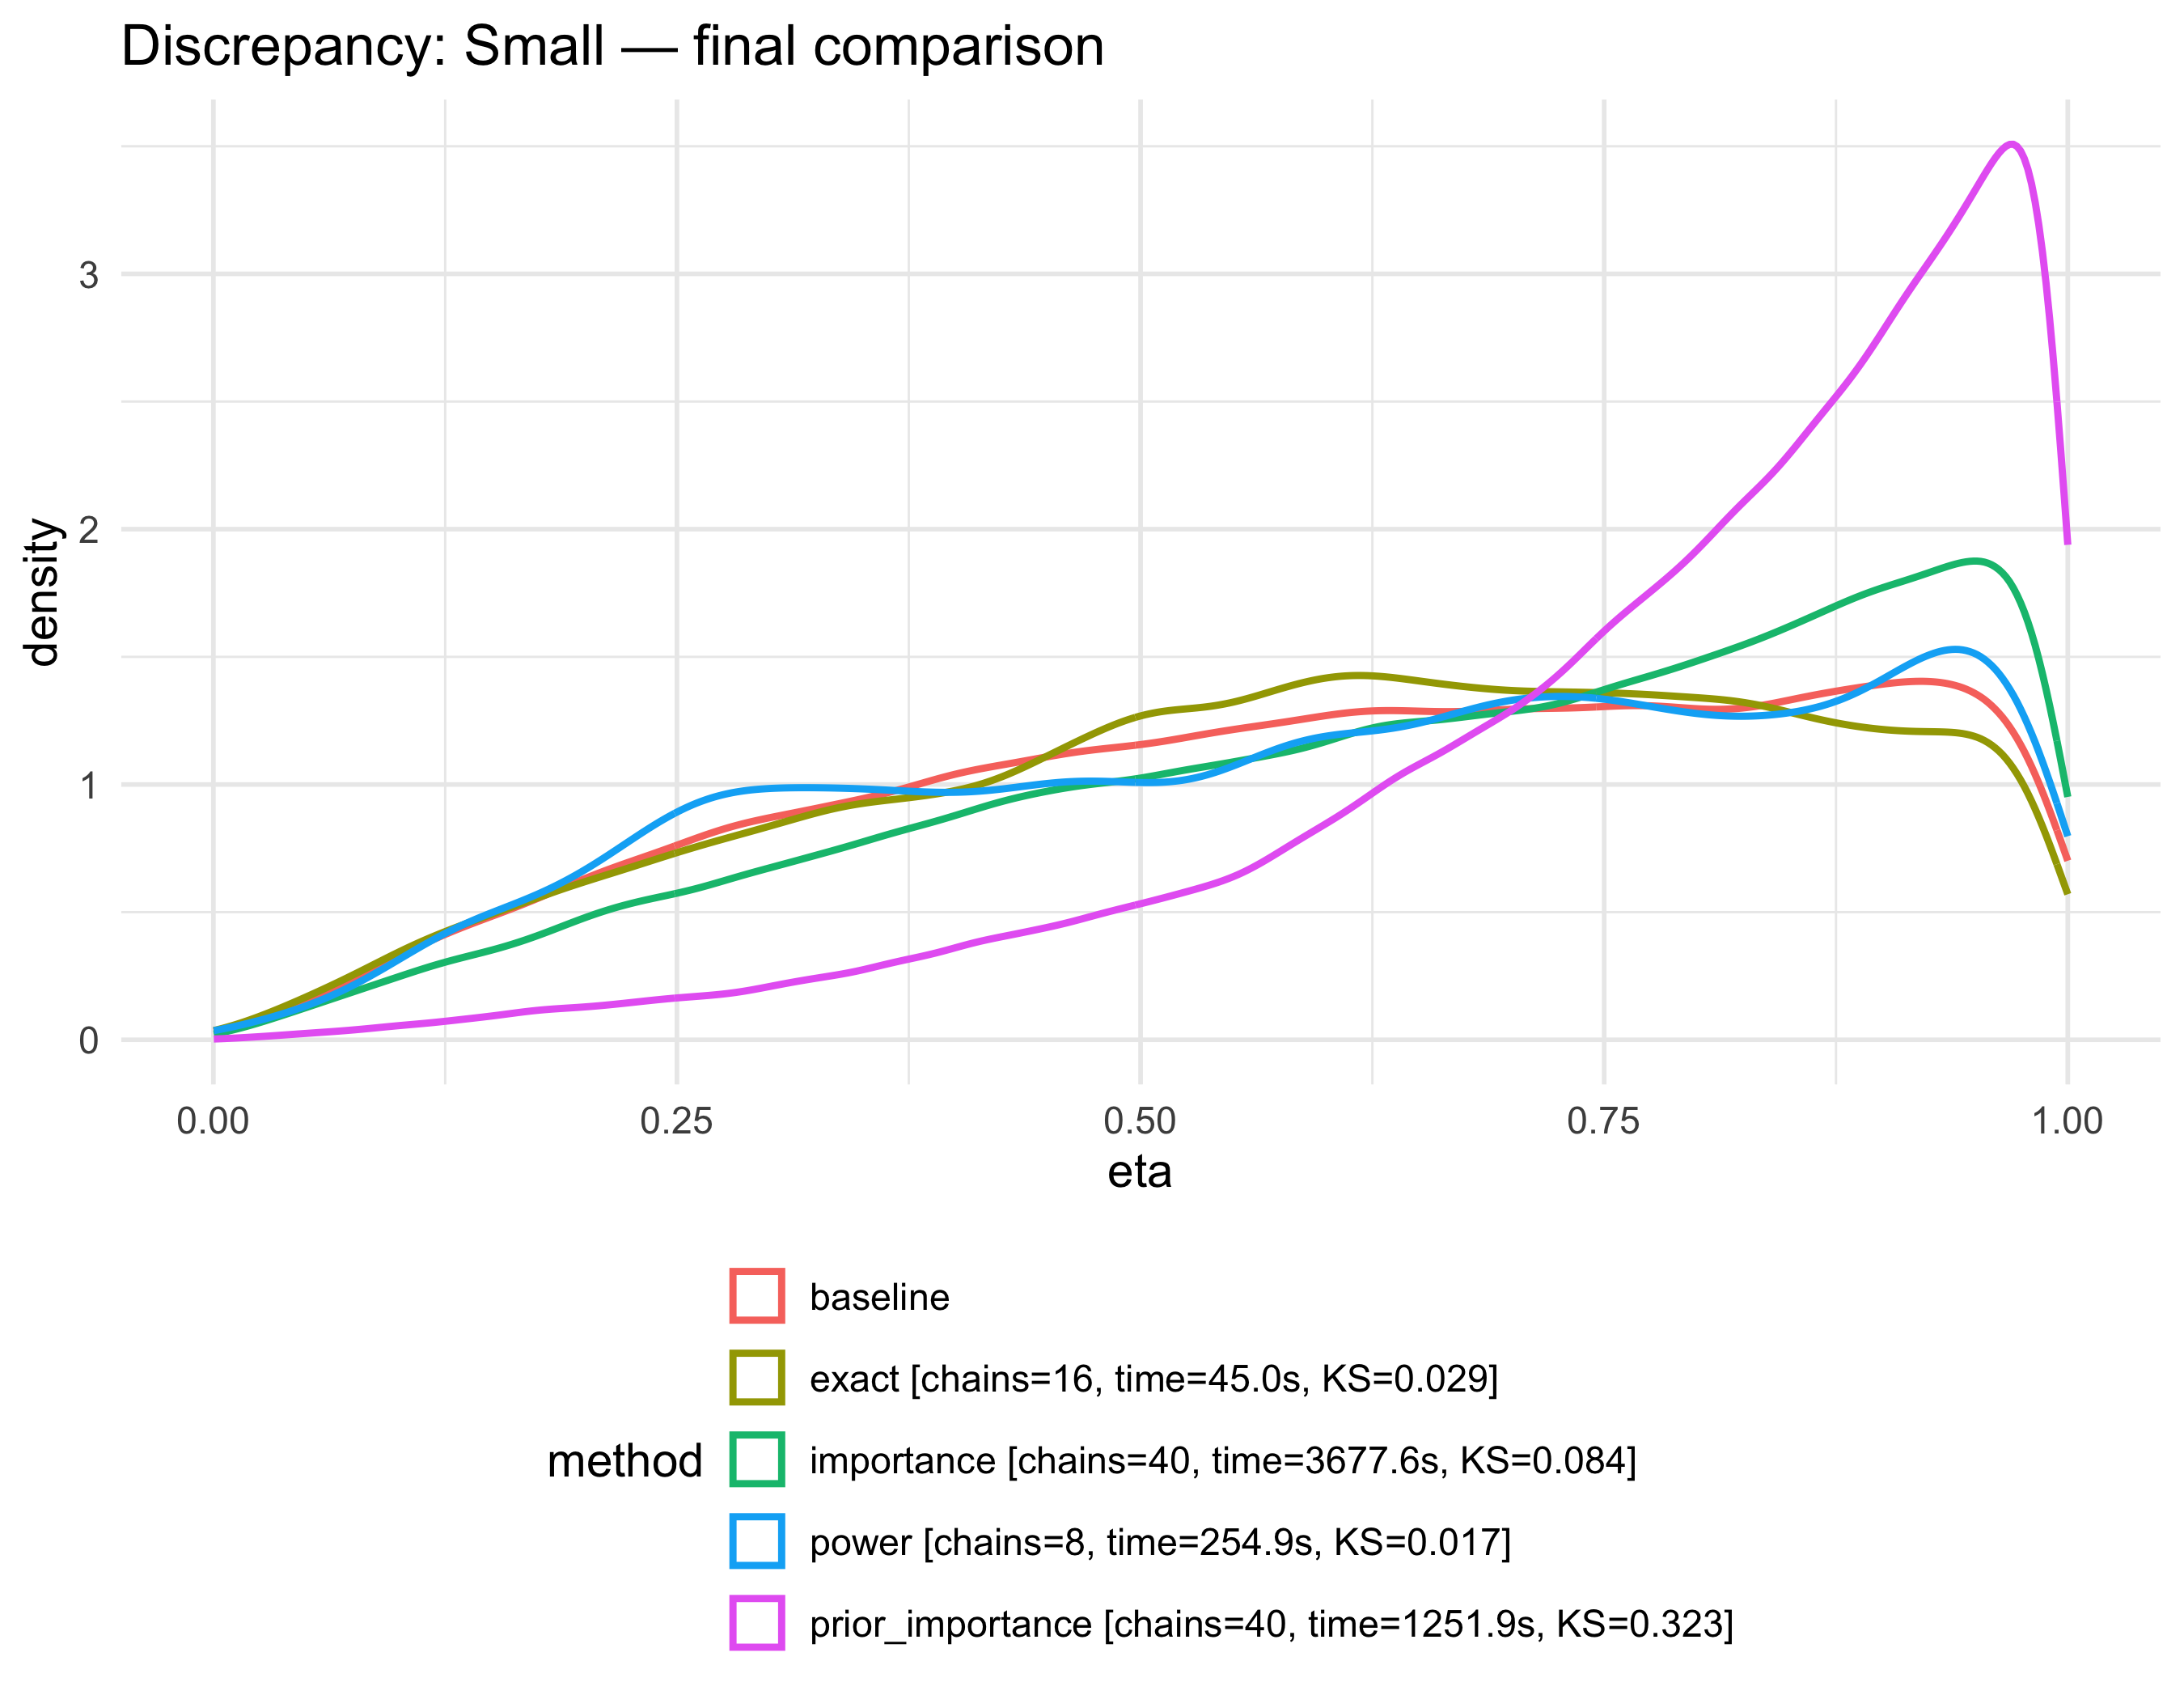
\includegraphics[width=\linewidth]{figures/ch5/convergence_small.png}
    \caption{Posterior densities for $\eta$ under low discrepancy ($\delta = 0.1$). Each approximate estimator label reports the total number of chains run, wall-clock time, and final KS distance to the Stan baseline.}
    \label{fig:convergence-small}
\end{figure}

\begin{figure}[H]
    \centering
    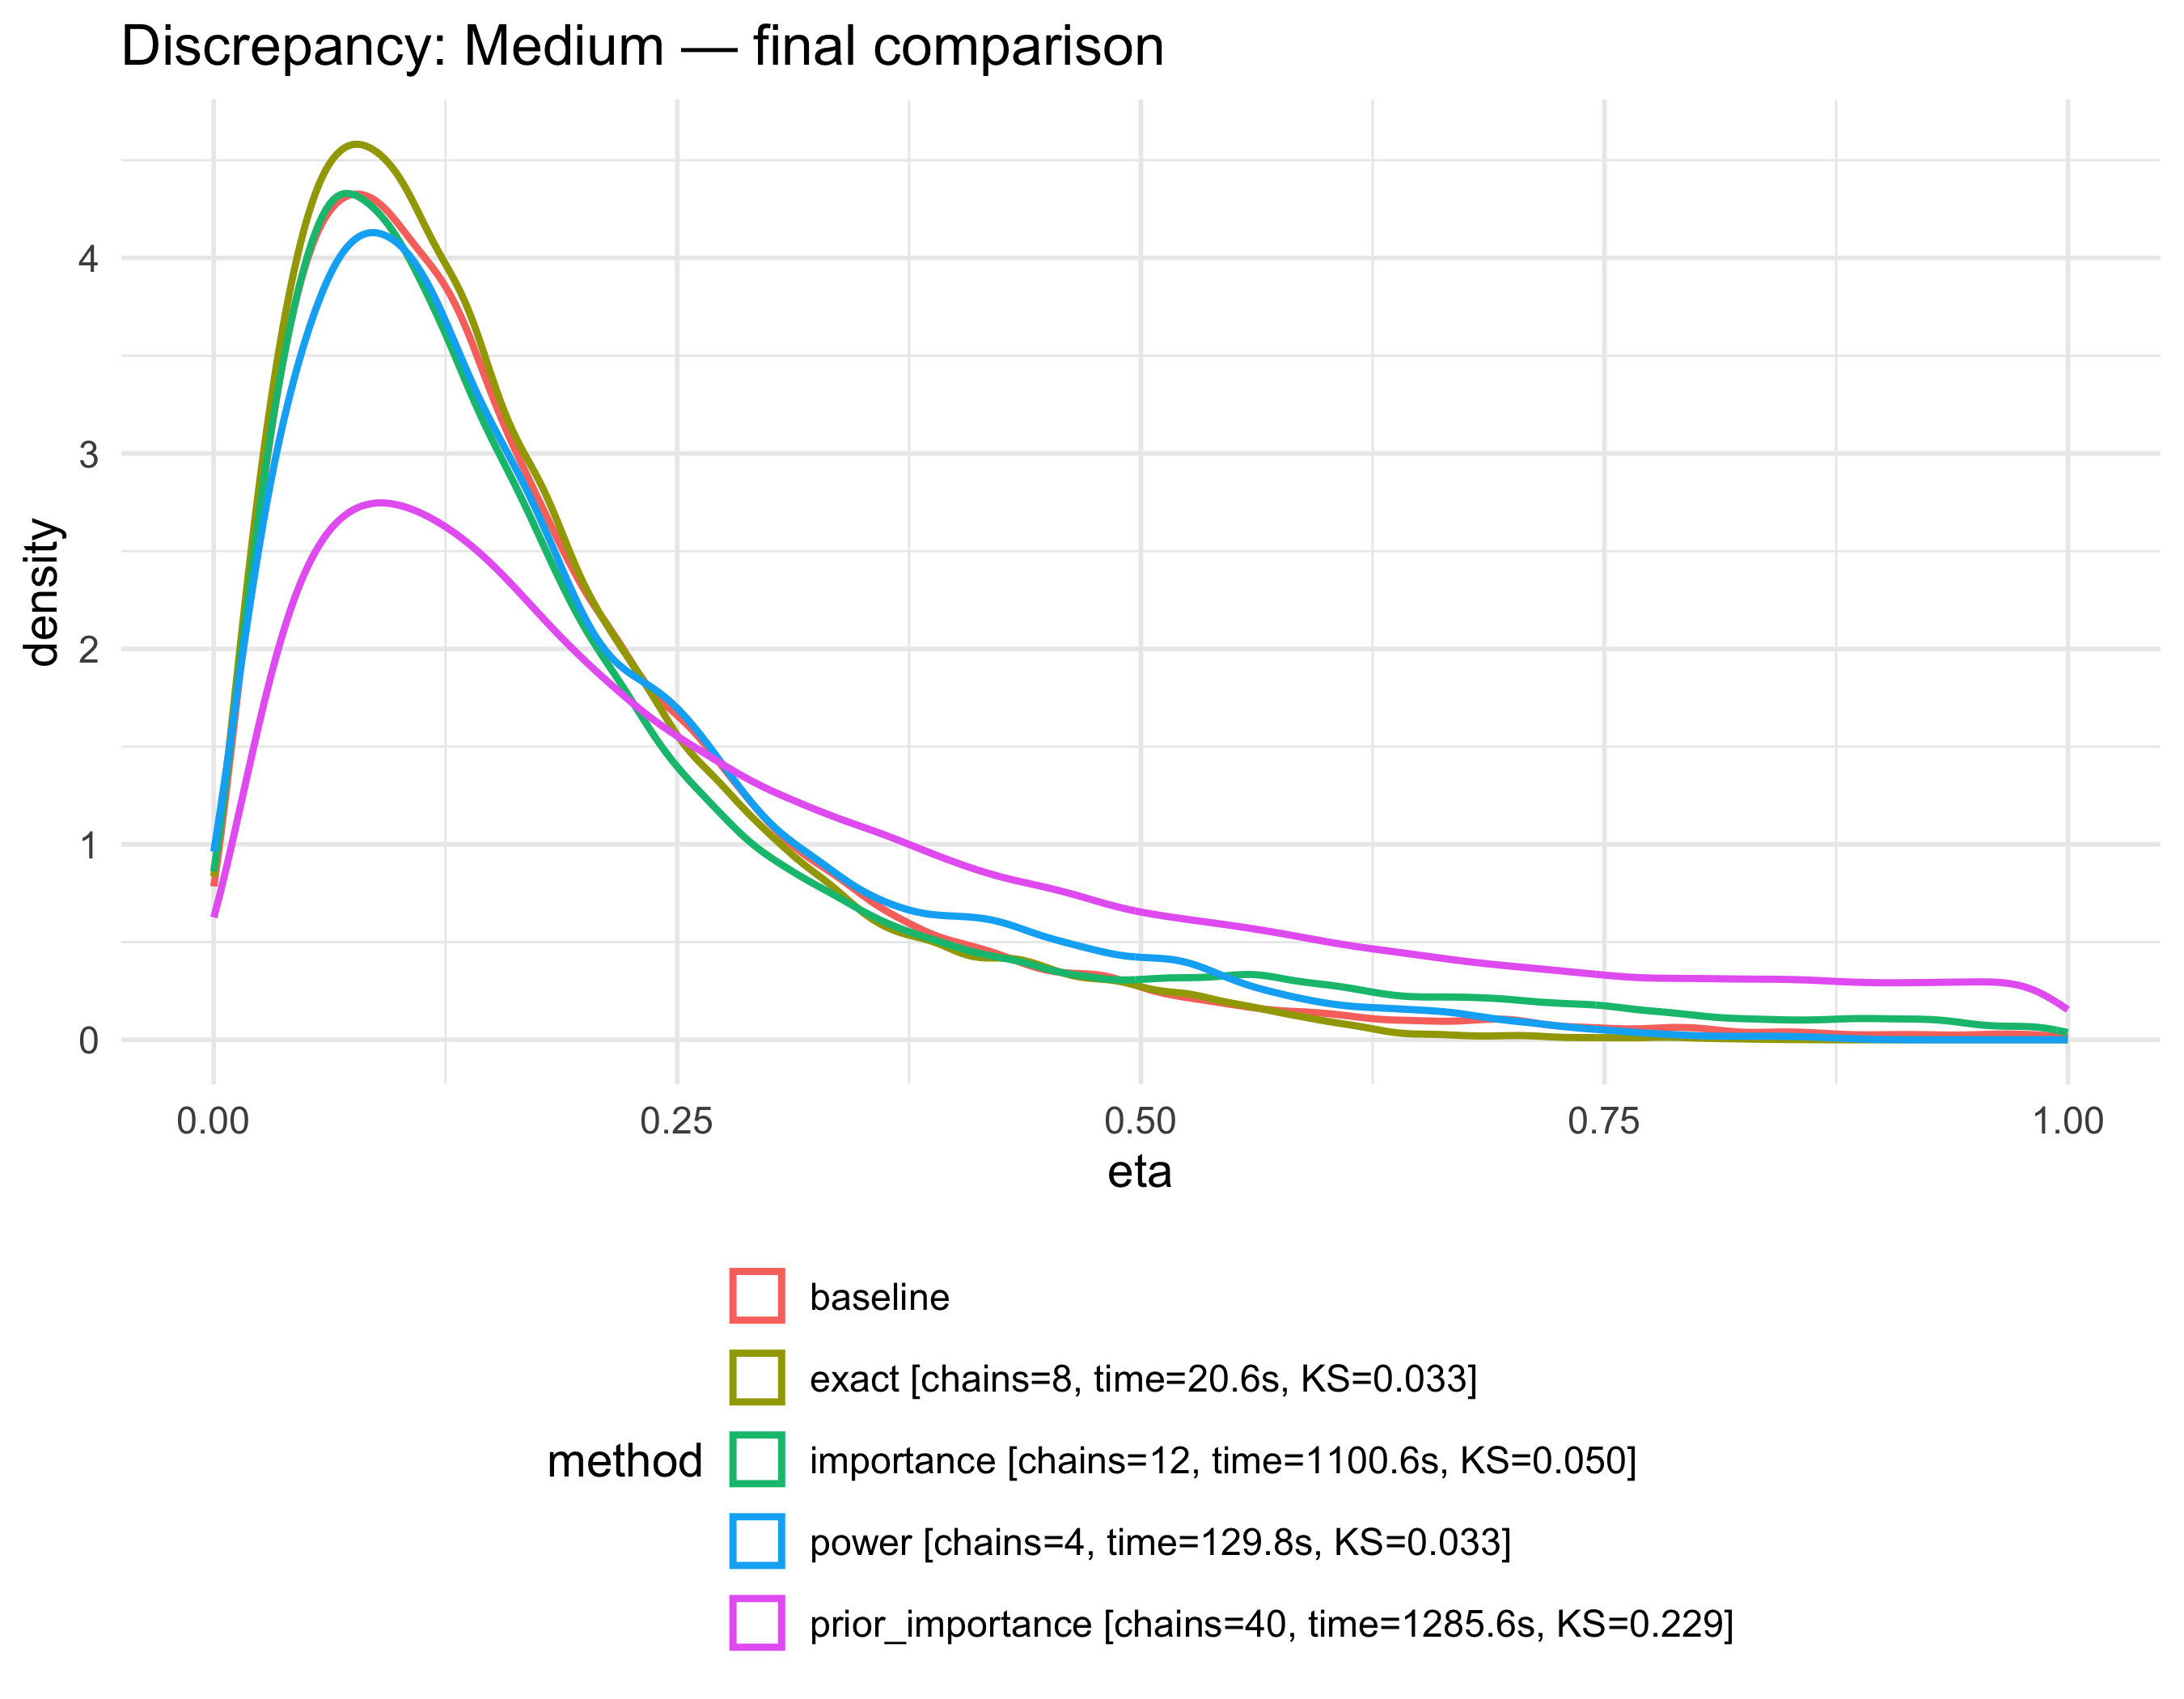
\includegraphics[width=\linewidth]{figures/ch5/convergence_medium.png}
    \caption{Posterior densities for $\eta$ under moderate discrepancy ($\delta = 0.5$).}
    \label{fig:convergence-medium}
\end{figure}

\begin{figure}[H]
    \centering
    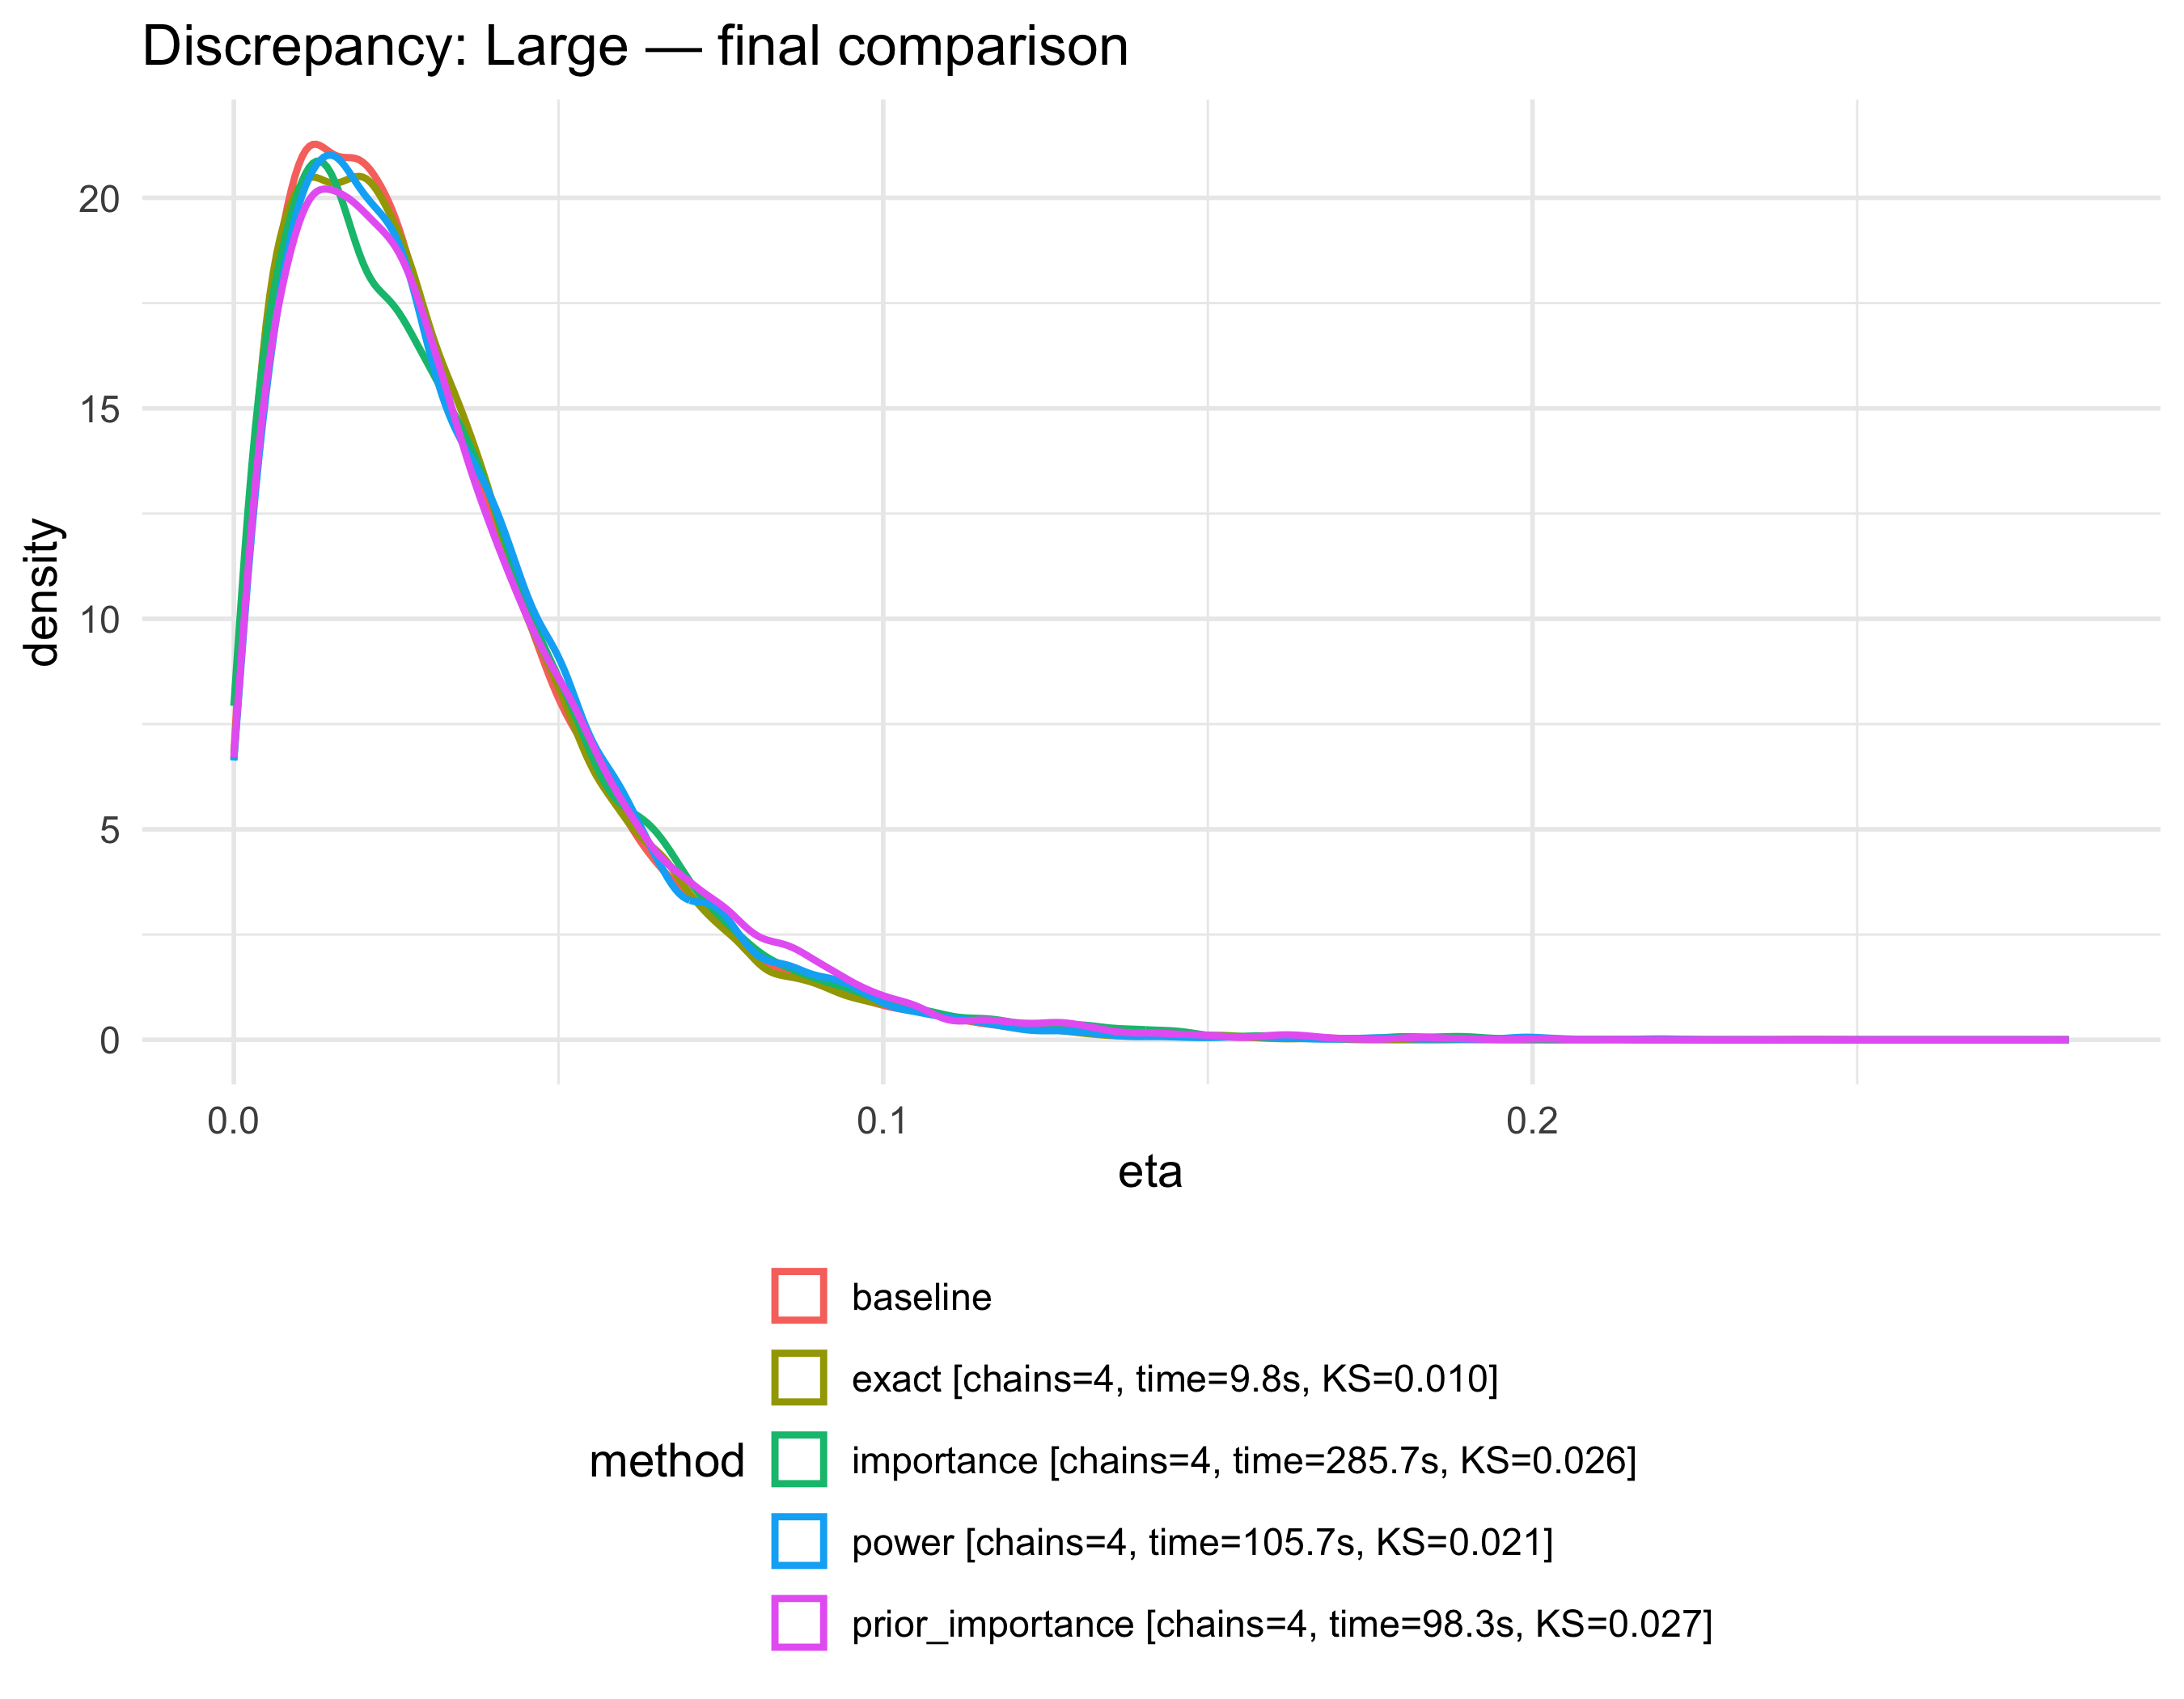
\includegraphics[width=\linewidth]{figures/ch5/convergence_large.png}
    \caption{Posterior densities for $\eta$ under high discrepancy ($\delta = 1.0$). Under strong conflict between datasets the posterior concentrates near zero and all methods converge in a single batch.}
    \label{fig:convergence-large}
\end{figure}

\begin{table}[ht]
    \centering
    \begin{tabular}{lcccccc}
    \hline
    & \multicolumn{2}{c}{Small ($\delta=0.1$)} & \multicolumn{2}{c}{Medium ($\delta=0.5$)} & \multicolumn{2}{c}{Large ($\delta=1.0$)} \\
    Method & Chains & KS & Chains & KS & Chains & KS \\
    \hline
    Exact             &  16 & 0.029 &  8 & 0.033 & 4 & 0.010 \\
    Prior-importance  &  40 & 0.323 & 40 & 0.229 & 4 & 0.027 \\
    Importance        &  40 & 0.084 & 12 & 0.050 & 4 & 0.026 \\
    Power             &   8 & 0.017 &  4 & 0.033 & 4 & 0.021 \\
    \hline
    \end{tabular}
    \caption{Total chains required and final KS distance to the Stan HMC baseline. A dash indicates the method reached 10 batches (40 chains) without satisfying the convergence criterion.}
    \label{tab:convergence-comparison}
\end{table}

\subsection{Discussion of results}

The results reveal a consistent pattern across discrepancy regimes.
Under low discrepancy (Figure~\ref{fig:convergence-small}), the posterior for $\eta$ spreads across a wide range, reflecting genuine uncertainty about how much weight to assign to the historical data.
In this regime the estimators differ most sharply: the power estimator converges in just two batches (8 chains, KS$=0.017$), the exact algorithm requires four batches (16 chains, KS$=0.029$), whereas the importance estimator exhausts all ten batches without reaching the threshold (KS$=0.084$) and the prior-importance estimator deviates substantially from the baseline (KS$=0.323$).
The inefficiency of $\delta_a$ here is expected: when the posterior for $\eta$ is diffuse, prior samples for $\theta$ are a poor proposal for the normalising-constant integral, yielding high-variance estimates of the log-ratio.

Under moderate discrepancy (Figure~\ref{fig:convergence-medium}), the posterior shifts toward smaller values of $\eta$, indicating the model has begun to down-weight the historical data.
The power estimator again converges in a single batch (4 chains), the exact algorithm in two, and the importance estimator in three.
The prior-importance estimator still fails to reach the threshold, though its KS distance has improved relative to the low-discrepancy case.

When the two datasets are in strong conflict (Figure~\ref{fig:convergence-large}), the posterior concentrates sharply near $\eta \approx 0$.
In this regime all four estimators converge in a single batch of four chains, and the KS distances are uniformly small.
The sharp concentration of the posterior makes the normalising-constant ratio easy to estimate regardless of the proposal, erasing the differences observed at lower discrepancy levels.

Overall, the power estimator is the most efficient of the three approximate methods: it matches or beats the exact algorithm in chains required across all scenarios.
The prior-importance estimator is consistently the weakest, particularly when the posterior is diffuse.
These findings suggest that the choice of estimator matters most in low-discrepancy settings, where the posterior for $\eta$ is broad and the normalising constant must be estimated accurately over a wide range of values.

\subsection{Linear regression with Normal-Inverse-Gamma priors}
\label{subsec:nig-lm-experiment}

We next consider a Gaussian linear regression model with unknown variance.
This experiment is designed to evaluate the exchange update in a setting where the normalized power prior remains analytically tractable, but the normalizing constant is no longer a simple linear function of the power parameter.
Let $D_0 = (\bfX_0,\bfy_0)$ denote the historical data and let $D = (\bfX,\bfy)$ denote the current data.
We assume
\begin{equation}
    \bfy_0 = \bfX_0 \bfbt + \bfeps_0,
    \qquad
    \bfy = \bfX \bfbt + \bfeps,
\end{equation}
where $\bfeps_0 \sim \cN(\bfzero,\sg \bfI_{n_0})$ and $\bfeps \sim \cN(\bfzero,\sg \bfI_n)$.
The variance $\sg$ is unknown.
The initial prior is Normal-Inverse-Gamma,
\begin{equation}
    \bfbt \mid \sg \sim \cN(\bfmu_0,\sg \bfV_0),
    \qquad
    \sg \sim \InvGam(a,b).
\end{equation}
For a fixed value of $\eta$, the powered prior is given by
\begin{equation}
    \pi_{\eta}(\bfbt,\sg \mid D_0)
    =
    \frac{
        L(D_0 \mid \bfbt,\sg)^\eta \pi_0(\bfbt,\sg)
    }{
        c_0(\eta)
    }.
\end{equation}
The normalizing constant is
\begin{equation}
    c_0(\eta)
    =
    \int_0^\infty
    \int_{\bR^p}
    L(D_0 \mid \bfu,v)^\eta
    \pi_0(\bfu,v)
    \dd \bfu
    \dd v.
\end{equation}
In this model, $c_0(\eta)$ is available in closed form by conjugacy.
This allows us to construct an analytic reference chain for $\eta$ and to validate algorithms that do not directly evaluate $c_0(\eta)$.
The marginal posterior density of $\eta$ is proportional to
\begin{equation}
    \pi(\eta \mid D_0,D)
    \propto
    \frac{
        \pi_A(\eta)
        \Gamma(n/2+\nu_0)
        \abs{\Lambda_0}^{1/2}
        H_0(\eta)^{\nu_0}
    }{
        \abs{\Lambda}^{1/2}
        \Gamma(\nu_0)
        H(\eta)^{\nu_0+n/2}
    }.
    \label{eq:nig-lm-eta-marginal}
\end{equation}
The quantities $\nu_0$, $\Lambda_0$, $H_0(\eta)$, $\Lambda$, and $H(\eta)$ are defined in Appendix~\ref{example:nig_lm}.
Although the analytic expression is available here, the exchange algorithm does not require evaluating $c_0(\eta)$.
Given the current state $(\bfbt,\sg,\eta)$, we propose $\eta'$ and draw an auxiliary value
\begin{equation}
    ({\bfbt}^\star,{\sg}^\star)
    \sim
    \pi_{\eta'}(\bfbt,\sg \mid D_0).
\end{equation}
The exchange log-ratio for the $\eta$ update is
\begin{align}
    \log R_{\mathrm{ex}}
    &=
    (\eta'-\eta)
    \log L(D_0 \mid \bfbt,\sg)
    +
    (\eta-\eta')
    \log L(D_0 \mid {\bfbt}^\star,{\sg}^\star)
    \nonumber
    \\
    &\quad
    +
    \log \frac{\pi_A(\eta')}{\pi_A(\eta)}
    +
    \log \frac{q(\eta \mid \eta')}{q(\eta' \mid \eta)}.
    \label{eq:nig-lm-exchange-log-ratio}
\end{align}
The proposal is then accepted with probability $\min\{1,\exp(\log R_{\mathrm{ex}})\}$.
When the auxiliary draw from $\pi_{\eta'}(\bfbt,\sg \mid D_0)$ is exact, this update has the correct invariant distribution for the normalized power prior.
This follows from the exchange algorithm for doubly-intractable distributions, where an auxiliary draw from the proposed normalized model cancels the unknown ratio of normalizing constants in the Metropolis-Hastings acceptance probability~\cite{murray2012}. 
The exchange algorithm therefore provides an exact update for $\eta$ under the powered-prior simulation assumption.
This assumption is satisfied in the present experiment because the powered prior is Normal-Inverse-Gamma.

We compare three methods.
The first method is an analytic Metropolis-Hastings reference that evaluates Equation~\eqref{eq:nig-lm-eta-marginal}.
The second method is the exchange Metropolis-Hastings update in Equation~\eqref{eq:nig-lm-exchange-log-ratio}.
The third method is a path-sampling pseudo-marginal method based on a Monte Carlo approximation of the normalizing constant ratio.
The path-sampling method is included as a computational baseline and is classified according to the exactness of the estimator used in its acceptance ratio.
If the estimator is not non-negative and unbiased for the required marginal target, the method is treated as approximate rather than exact.
This distinction follows the pseudo-marginal principle, where exactness requires a non-negative unbiased estimator of the target density on an extended space~\cite{andrieu2009}.

We generate three discrepancy scenarios between the historical and current regression coefficients.
In the small-discrepancy scenario, the current coefficient vector is close to the historical coefficient vector.
In the medium-discrepancy scenario, the current coefficient vector is moderately shifted.
In the large-discrepancy scenario, the current coefficient vector is substantially shifted.
The expected qualitative behavior is that the posterior distribution of $\eta$ moves toward smaller values as the discrepancy increases.
This reflects reduced borrowing from the historical data when the historical and current data-generating mechanisms are less compatible.

The main diagnostic is the one-dimensional Wasserstein distance from each method to the analytic reference.
We report this distance separately for $\eta$, $\norm{\bfbt}_2$, and $\sg$.
We also report posterior means, posterior standard deviations, effective sample sizes, acceptance rates, and runtime.
The norm $\norm{\bfbt}_2$ summarizes the magnitude of the regression coefficient vector, while $\sg$ is reported separately because it represents the residual variance and should not be combined with $\bfbt$ into a single geometric average.

\begin{figure}[ht]
    \centering
    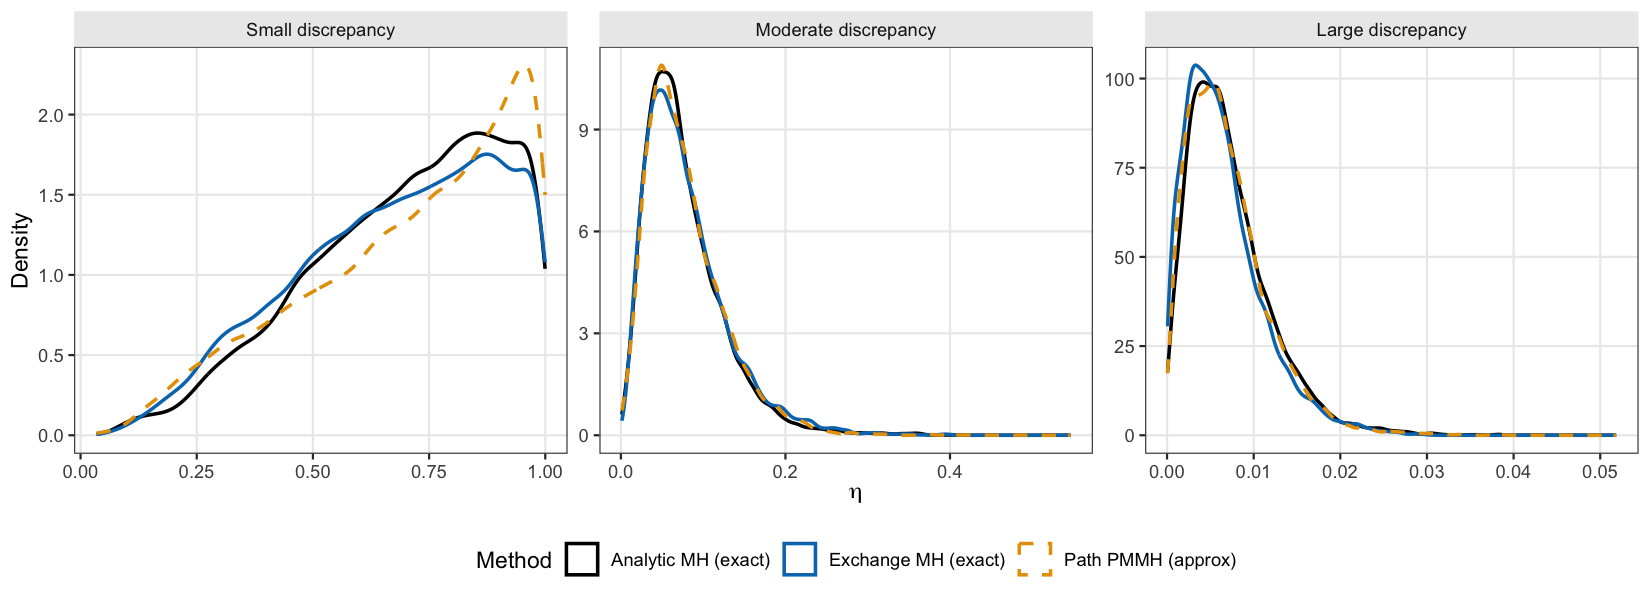
\includegraphics[width=\textwidth]{../software/experiments/results/nig_lm_exchange/posterior_eta_all_discrepancies.png}
    \caption{Posterior density of $\eta$ for the linear regression NPP experiment across discrepancy scenarios.}
    \label{fig:nig-lm-eta-density}
\end{figure}

\begin{figure}[ht]
    \centering
    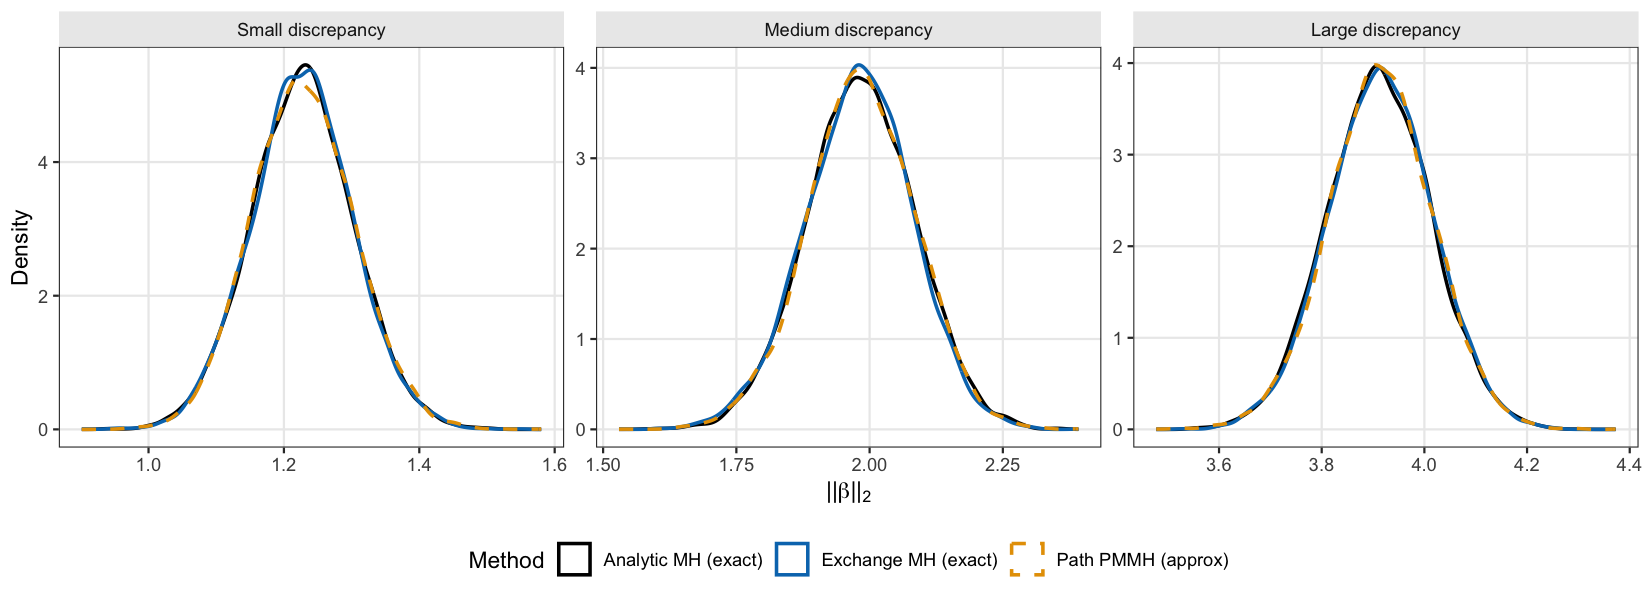
\includegraphics[width=\textwidth]{../software/experiments/results/nig_lm_exchange/posterior_beta_norm_all_discrepancies.png}
    \caption{Posterior density of $\norm{\bfbt}_2$ for the linear regression NPP experiment across discrepancy scenarios.}
    \label{fig:nig-lm-beta-norm-density}
\end{figure}

\begin{figure}[ht]
    \centering
    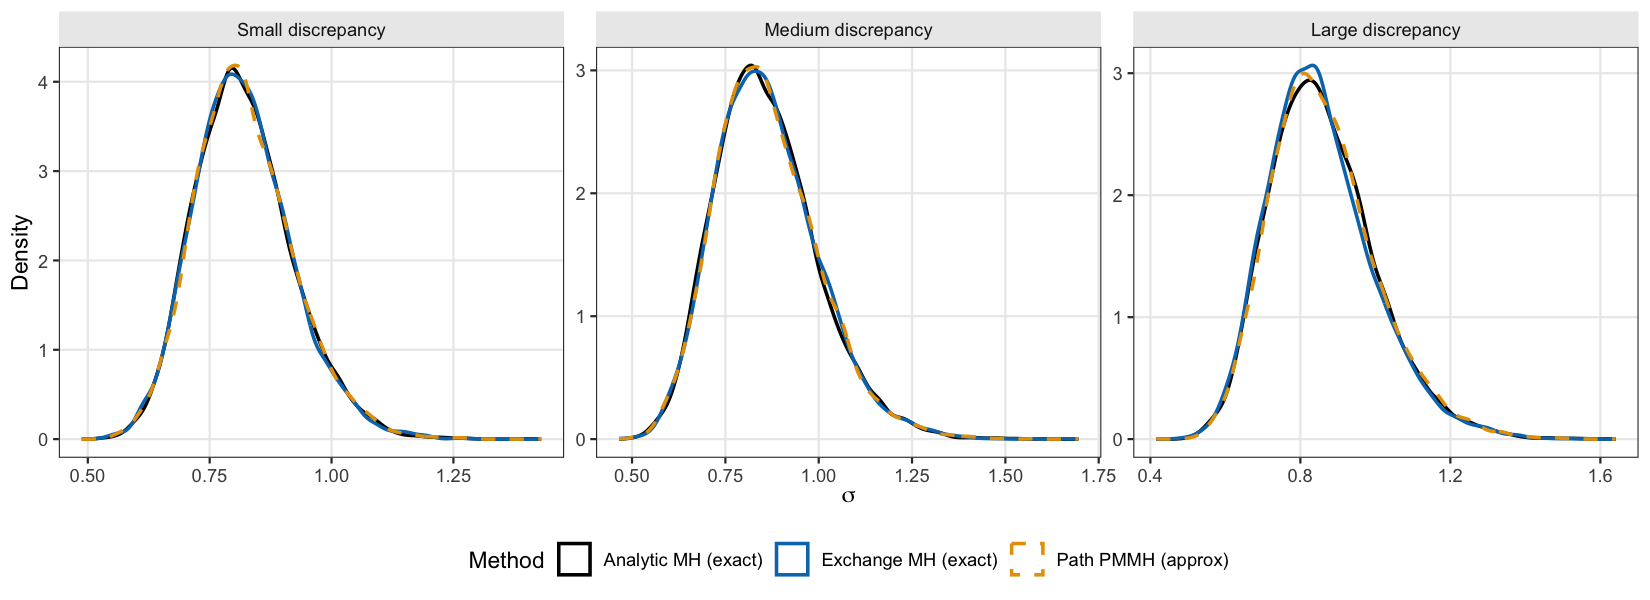
\includegraphics[width=\textwidth]{../software/experiments/results/nig_lm_exchange/posterior_sigma_all_discrepancies.png}
    \caption{Posterior density of $\sg$ for the linear regression NPP experiment across discrepancy scenarios.}
    \label{fig:nig-lm-sigma-density}
\end{figure}

\begin{table}[ht]
  \centering
  \begin{tabular}{llcccccc}
  \hline
  Scenario & Method & $W_\eta$ & $W_{\|\beta\|}$ & $W_\sigma$ & ESS$_\eta$ & Acc.\ $\eta$ & Time (s) \\
  \hline
  Small & Analytic MH & 0.000 & 0.000 & 0.000 & 195 & 0.928 & 3.1 \\
  Small & Exchange MH & 0.019 & 0.001 & 0.002 & 222 & 0.902 & 1.6 \\
  Small & Path PMMH & 0.022 & 0.001 & 0.001 & 199 & 0.913 & 31.6 \\
  \hline
  Moderate & Analytic MH & 0.000 & 0.000 & 0.000 & 717 & 0.859 & 3.2 \\
  Moderate & Exchange MH & 0.003 & 0.003 & 0.002 & 557 & 0.797 & 1.6 \\
  Moderate & Path PMMH & 0.002 & 0.001 & 0.002 & 797 & 0.837 & 32.5 \\
  \hline
  Large & Analytic MH & 0.000 & 0.000 & 0.000 & 682 & 0.863 & 3.1 \\
  Large & Exchange MH & 0.001 & 0.003 & 0.009 & 577 & 0.824 & 1.6 \\
  Large & Path PMMH & 0.000 & 0.003 & 0.003 & 694 & 0.858 & 32.1 \\
  \hline
  \end{tabular}
  \caption{Diagnostic comparison for the linear regression NPP experiment with Normal-Inverse-Gamma priors. Wasserstein distances are computed against the analytic MH baseline within each discrepancy scenario.}
  \label{tab:nig-lm-exchange-diagnostics}
\end{table}


\begin{table}[ht]
  \centering
  \begin{tabular}{llcccccc}
  \hline
  Scenario & Method & $\bar{\eta}$ & $\mathrm{sd}(\eta)$ & $\overline{\|\beta\|}$ & $\mathrm{sd}(\|\beta\|)$ & $\bar{\sigma}$ & $\mathrm{sd}(\sigma)$ \\
  \hline
  Small & Analytic MH & 0.697 & 0.208 & 1.227 & 0.076 & 0.820 & 0.101 \\
  Small & Exchange MH & 0.679 & 0.217 & 1.228 & 0.075 & 0.818 & 0.101 \\
  Small & Path PMMH & 0.705 & 0.227 & 1.229 & 0.075 & 0.821 & 0.101 \\
  \hline
  Medium & Analytic MH & 0.077 & 0.049 & 1.984 & 0.102 & 0.862 & 0.137 \\
  Medium & Exchange MH & 0.080 & 0.051 & 1.981 & 0.101 & 0.863 & 0.137 \\
  Medium & Path PMMH & 0.078 & 0.047 & 1.983 & 0.102 & 0.863 & 0.138 \\
  \hline
  Large & Analytic MH & 0.007 & 0.005 & 3.912 & 0.102 & 0.863 & 0.142 \\
  Large & Exchange MH & 0.007 & 0.005 & 3.915 & 0.101 & 0.854 & 0.140 \\
  Large & Path PMMH & 0.007 & 0.005 & 3.915 & 0.103 & 0.860 & 0.141 \\
  \hline
  \end{tabular}
  \caption{Posterior summaries for the NIG linear regression NPP experiment.}
  \label{tab:nig-lm-exchange-summaries}
\end{table}


\chapter{Discussion}

\subparagraph*{Code Availability} The code is available at: \url{https://github.com/adamesalles/npp-msc-thesis}. 



% ----------------------------------------------------------
% Referências bibliográficas
% ----------------------------------------------------------
\citeoption{abnt-etal-list=5}
\bibliographystyle{abntex2-cite-min}
\bibliography{bibliography}



% ----------------------------------------------------------
% Glossário
% ----------------------------------------------------------
%
% Consulte o manual da classe abntex2 para orientações sobre o glossário.
%
%\glossary

% ----------------------------------------------------------
% Apêndices
% ----------------------------------------------------------

% ---
% Inicia os apêndices
% ---
\begin{apendicesenv}

% Imprime uma página indicando o início dos apêndices
%\partapendices

% ----------------------------------------------------------
\chapter{Proofs}

\section{Thermodynamic identity for the normalising constant}
\label{proof:deriv-normalising-constant}

\begin{proof}
Under regularity conditions permitting differentiation under the integral sign, we have
\begin{align}
    \dv{c_0(\eta)}{\eta}
    &= \dv{}{\eta} \int_{\Theta} L_0(D_0 \mid t)^{\eta}\, \dd P_0(t) \\
    &= \int_{\Theta} \dv{}{\eta} L_0(D_0 \mid t)^{\eta}\, \dd P_0(t) \\
    &= \int_{\Theta} \log L_0(D_0 \mid t)\cdot L_0(D_0 \mid t)^{\eta}\, \dd P_0(t) \\
    &= c_0(\eta) \int_{\Theta} \log L_0(D_0 \mid t)\cdot \pi_\eta(t \mid D_0)\, \dd t \\
    &= c_0(\eta)\, \bE_{\pi_\eta}\bigl[\log L_0(D_0 \mid \theta)\bigr].
\end{align}
Since $c_0(\eta) > 0$ whenever the initial prior is proper, dividing both sides by $c_0(\eta)$ yields \eqref{eq:normalising-constant-log}.
\end{proof}

\section{Unbiasedness of the Poisson estimator}
\label{proof:poisson-unbiased}

\begin{proof}
We use the notation of Section~\ref{subsec:poisson-estimator}: write $\lambda \coloneqq \lambda_{\eta,\eta'}$, $c \coloneqq c_{\eta,\eta'}$, and $\Delta \coloneqq \Delta(\eta,\eta')$.
Since $(U_j, \theta_j) \overset{\mathrm{iid}}{\sim} \mathsf{P}_{\eta,\eta'}$ and $K \sim \mathrm{Poisson}(\lambda)$ are drawn independently, the tower property gives
\begin{align}
    \bE\bigl[\widehat{I}(\eta,\eta')\bigr]
    &= \exp\{\lambda - c\}\,
    \bE_K\!\left[
        \left(
            \bE_{\mathsf{P}_{\eta,\eta'}}
            \!\left[\frac{c - Z_{\eta,\eta'}}{\lambda}\right]
        \right)^{\!K}
    \right] \\
    &= \exp\{\lambda - c\}\,
    \bE_K\!\left[\left(\frac{c - \Delta}{\lambda}\right)^{\!K}\right].
\end{align}
Applying the probability-generating function of a $\mathrm{Poisson}(\lambda)$ random variable, $\bE[r^K] = \exp\{\lambda(r-1)\}$, with $r = (c - \Delta)/\lambda$, gives
\begin{align}
    \bE\bigl[\widehat{I}(\eta,\eta')\bigr]
    &= \exp\{\lambda - c\}
    \cdot
    \exp\!\left\{\lambda\!\left(\frac{c - \Delta}{\lambda} - 1\right)\right\} \\
    &= \exp\{\lambda - c\}
    \cdot \exp\{c - \Delta - \lambda\} \\
    &= \exp\{-\Delta\}
    = \frac{c_0(\eta)}{c_0(\eta')},
\end{align}
which establishes the claim.
\end{proof}

\section{Correctness of the exchange algorithm}
\label{proof:exchange-correctness}

\begin{proof}
We verify detailed balance for the augmented kernel.
Let $\pi(\eta \mid \theta) \propto \pi_A(\eta)\, L_0(D_0 \mid \theta)^\eta / c_0(\eta)$ denote the conditional target for $\eta$.
The exchange algorithm augments the state space with $\theta^\star$ drawn from the proposed normalised model:
\begin{equation}
    \theta^\star \sim \pi_{\eta'}(\theta \mid D_0)
    =
    \frac{L_0(D_0 \mid \theta)^{\eta'}}{c_0(\eta')}\,\pi_0(\theta).
\end{equation}
The augmented target on $(\eta, \theta^\star)$ is
\begin{equation}
    \widetilde\pi(\eta, \theta^\star)
    \propto
    \pi(\eta \mid \theta)\cdot \pi_{\eta'}(\theta^\star \mid D_0).
\end{equation}
The proposed move $(\eta, \theta^\star) \to (\eta', \theta)$ is accepted with the Metropolis--Hastings ratio
\begin{align}
    R_{\mathrm{ex}}
    &=
    \frac{\widetilde\pi(\eta', \theta)\, q(\eta \mid \eta')}
         {\widetilde\pi(\eta, \theta^\star)\, q(\eta' \mid \eta)}
    =
    \frac{\pi_A(\eta')\, L_0(D_0 \mid \theta)^{\eta'} / c_0(\eta')}
         {\pi_A(\eta)\, L_0(D_0 \mid \theta)^{\eta} / c_0(\eta)}
    \cdot
    \frac{L_0(D_0 \mid \theta)^{\eta} / c_0(\eta)}
         {L_0(D_0 \mid \theta^\star)^{\eta'} / c_0(\eta')}
    \cdot
    \frac{q(\eta \mid \eta')}{q(\eta' \mid \eta)}.
\end{align}
The factors $c_0(\eta)$ and $c_0(\eta')$ cancel, yielding
\begin{equation}
    R_{\mathrm{ex}}
    =
    \frac{\pi_A(\eta')}{\pi_A(\eta)}
    \cdot
    \frac{q(\eta \mid \eta')}{q(\eta' \mid \eta)}
    \cdot
    \frac{L_0(D_0 \mid \theta)^{\eta' - \eta}}
         {L_0(D_0 \mid \theta^\star)^{\eta' - \eta}},
\end{equation}
which is exactly the ratio in Section~\ref{sec:exact-exchange}.
The augmented kernel therefore satisfies detailed balance with respect to $\widetilde\pi$.
It remains to verify that the marginal of $\widetilde\pi$ over $\theta^\star$ equals the desired target $\pi(\eta \mid \theta)$.
Indeed,
\begin{align}
    \int_\Theta \widetilde\pi(\eta, \theta^\star) \, \dd\theta^\star
    &\propto
    \pi(\eta \mid \theta)
    \int_\Theta \pi_{\eta'}(\theta^\star \mid D_0) \, \dd\theta^\star
    =
    \pi(\eta \mid \theta),
\end{align}
since $\pi_{\eta'}(\cdot \mid D_0)$ is a proper probability density integrating to one.
Hence the marginal invariant distribution of $\eta$ under the augmented kernel is $\pi(\eta \mid \theta)$, as required.
\end{proof}

\section{Convexity of log-normalising constant}
\label{proof:log-c0-convex}

\begin{proof}
We show that $\eta \mapsto \log c_0(\eta)$ is convex on $[0,1]$.
By \eqref{eq:normalising-constant-log}, the second derivative satisfies
\begin{equation}
    \dv[2]{\log c_0(\eta)}{\eta}
    =
    \dv{}{\eta}\, \bE_{\pi_\eta}\bigl[\log L_0(D_0 \mid \theta)\bigr]
    =
    \mathrm{Var}_{\pi_\eta}\bigl[\log L_0(D_0 \mid \theta)\bigr]
    \geq
    0,
\end{equation}
where the identity follows by differentiating under the integral sign and recognising the resulting expression as a variance under $\pi_\eta$.
Since the second derivative is non-negative, $\log c_0(\eta)$ is convex.
\end{proof}
% ----------------------------------------------------------
% \input{src/appendice}

% ----------------------------------------------------------
%\chapter{Nullam elementum urna vel imperdiet sodales elit ipsum pharetra ligula
%ac pretium ante justo a nulla curabitur tristique arcu eu metus}
% ----------------------------------------------------------
%\lipsum[55-57]

\end{apendicesenv}
% ---


% ----------------------------------------------------------
% Anexos
% ----------------------------------------------------------

% ---
% Inicia os anexos
% ---
%\begin{anexosenv}

% Imprime uma página indicando o início dos anexos
%\partanexos


%\end{anexosenv}

%---------------------------------------------------------------------
% INDICE REMISSIVO
%---------------------------------------------------------------------
\phantompart
\printindex
%---------------------------------------------------------------------

\end{document}